%\documentclass[preprint]{aastex}  % USE THIS TO MAKE BIB, THEN FORMAT USING EMULATEAPJ
\documentclass[twocolumn,numberedappendix]{emulateapj} \shorttitle{PSA64}
\shortauthors{Ali, et al.}

\usepackage{amsmath} \usepackage{graphicx} \usepackage[figuresright]{rotating}
%\usepackage{rotating}
\usepackage{natbib}
%\usepackage{pdflscape} \usepackage{lscape}
\citestyle{aa}

\def\b{\mathbf{b}} \def\k{\mathbf{k}} \def\r{\mathbf{r}} \def\q{\mathbf{q}}
\def\b{\mathbf{b}} \def\kp{\mathbf{k}^\prime}
\def\kpp{\mathbf{k}^{\prime\prime}} \def\V{\mathbb{V}} \def\expval#1{\langle #1
\rangle} \def\At{\tilde{A}} \def\Vt{\tilde{V}} \def\Tt{\tilde{T}}
\def\tb{\langle T_b\rangle} \newcommand{\vis}{\mathbf{v}}
\newcommand{\x}{\mathbf{x}} \newcommand{\xhat}{\hat{\mathbf{x}}}
\newcommand{\A}{\mathbf{A}} \newcommand{\N}{\mathbf{N}}
\newcommand{\C}{\mathbf{C}} \newcommand{\Q}{\mathbf{Q}}
\newcommand{\rhat}{\hat{\mathbf{r}}}
\newcommand{\phat}{\hat{\mathbf{p}}}
\newcommand{\qhat}{\hat{\mathbf{q}}}
\newcommand{\hMpci}{h\ {\rm Mpc}^{-1}}
\newcommand{\Tsys}{T_{\rm sys}}
\newcommand{\Tspin}{T_{\rm s}}
\newcommand{\kmin}{k_{\rm min}}
\newcommand{\kmax}{k_{\rm max}}
\newcommand{\Tcmb}{T_\gamma}
\newcommand\abs[1]{\left|#1\right|}

\newcount\colveccount
\newcommand*\colvec[1]{
        \global\colveccount#1
        \begin{pmatrix}
        \colvecnext
}
\def\colvecnext#1{
        #1
        \global\advance\colveccount-1
        \ifnum\colveccount>0
                \\
                \expandafter\colvecnext
        \else
                \end{pmatrix}
        \fi
}


\begin{document}

\title{PAPER-64 Power Spectrum: XXX a better title}

\author{
Zaki S. Ali\altaffilmark{1}, 
Aaron R. Parsons\altaffilmark{1,2}, 
Haoxuan Zheng\altaffilmark{12},
James E. Aguirre\altaffilmark{4},
Richard F. Bradley\altaffilmark{5,6,7},
Gianni Bernardi\altaffilmark{3}, 
Chris L. Carilli\altaffilmark{8,11},
Carina Cheng\altaffilmark{1},
David R. DeBoer\altaffilmark{2}, 
Matthew R. Dexter\altaffilmark{2},
%Steven R. Furlanetto\altaffilmark{XXX},
Daniel C. Jacobs\altaffilmark{9}, 
Pat Klima\altaffilmark{6},
Adrian Liu\altaffilmark{1}, 
David H. E. MacMahon\altaffilmark{2},
David F. Moore\altaffilmark{3},
Jonathan C. Pober\altaffilmark{10}, 
Nima Razavi\altaffilmark{11},
Irina I. Stefan\altaffilmark{11},
William P. Walbrugh\altaffilmark{3},
Andre Walker\altaffilmark{3}
}
% XXX more on author list
% XXX ordering of affil marks
%include Jasper Horrell, Jasper Grobbelaar, Matthys Maree
%\tableofcontents

\altaffiltext{1}{Astronomy Dept., U. California, Berkeley, CA}
\altaffiltext{2}{Radio Astronomy Lab., U. California, Berkeley, CA}
\altaffiltext{3}{Square Kilometer Array, South Africa Project, Cape Town, South Africa}
\altaffiltext{4}{Dept. of Physics and Astronomy, U. Pennsylvania, Philadelphia, PA} 
\altaffiltext{5}{Dept. of Electrical and Computer Engineering, U. Virginia, Charlottesville, VA}
\altaffiltext{6}{National Radio Astronomy Obs., Charlottesville, VA}
\altaffiltext{7}{Dept. of Astronomy, U. Virginia, Charlottesville, VA}
\altaffiltext{8}{National Radio Astronomy Obs., Socorro, NM}
\altaffiltext{9}{School of Earth and Space Exploration, Arizona State U., Tempe, AZ}
\altaffiltext{10}{Physics Dept.  U. Washington, Seattle, WA}
\altaffiltext{11}{Cavendish Lab., Cambridge, UK}
\altaffiltext{12}{Dept. of Physics, Massachusetts Institute of Technology,
Cambridge, MA}

\begin{abstract}
In this paper, we report new limits on 21cm emission from cosmic reionization
based on a 4.5-month observing campaign with a 64-element deployment of the
Donald C. Backer Precision Array for Probing the Epoch of Reionization (PAPER)
in South Africa.  This work extends the work presented in
\citet{parsons_et_al2014} with more collecting area, improved redundancy-based
calibration, optimal fringe-rate filtering, and improved power-spectral
analysis using optimal quadratic estimators. The result is a new $2\sigma$
upper limit on $\Delta^2(k)$ of ($20.6~{\rm mK})^2$ in the range
$0.1<k<0.5\hMpci$ at $z=8.4$.  This represents a four-fold improvement over the
previous best upper limit.  As we discuss in more depth in the companion to
this paper \citet{pober_et_al2015}, this upper limit supports and extends
previous evidence for significant heating in the intergalactic medium prior to
reionization. We conclude with a discussion of implications for future 21cm
reionization experiments, including the newly funded Hydrogen Epoch of
Reionization Array (HERA).  
\end{abstract}

\section{Introduction}

The {\it cosmic dawn} of the universe, which begins with the birth of the first stars and ends approximately
one billion years later with the full
reionization of the intergalactic medium (IGM), represents one of the last 
unexplored phases in cosmic history. 
Studying the formation of the first galaxies and their influence on the primordial IGM during this
period is among the highest priorities in modern astronomy.
During our cosmic dawn, IGM characteristics depend on the matter density field, the mass and clustering of 
the first galaxies \citep{lidz_et_al2008} [XXX check], their ultraviolet luminosities [XXX],
the abundance of X-ray sources and other sources of heating \citep{mesinger_et_al2013} [XXX check],
and higher-order cosmological effects like the relative velocities of baryons and dark matter \citep{visbal_et_al2012}.

Recent measurements
have pinned down the bright end of the galaxy luminosity function
at $z \la 8$ \citep{bouwens_et_al2010,schenker_et_al2013} and have detected a few sources at even greater
distances \citep{ellis_et_al2013,oesch_et_al2013}. 
In parallel, a number of indirect techniques have constrained the evolution of the neutral fraction
with redshift. Examples include integral constraints on reionization from the
optical depth of Thomson scattering to the CMB \citep{planck_et_al2014,planck_et_al2015},
large-scale CMB polarization anisotropies \citep{page_et_al2007}, and
secondary temperature fluctuations generated by the kinetic Sunyaev-Zel'dovich effect \citep{zahn_et_al2012,mesinger_et_al2012,george_et_al2014}.
Other probes of the tail end of reionization include
observations of resonant scattering of Ly$\alpha$ by the neutral IGM toward
distant quasars (the `Gunn-Peterson' effect) \citep{fan_et_al2006},
the demographics of Ly$\alpha$ emitting galaxies \citep{schenker_et_al2013,treu_et_al2013,Faisst_et_al2014},
and the
Ly$\alpha$ absorption profile toward very distant quasars \citep{bolton_et_al2011}.
As stands, the known population of galaxies falls well short 
of the requirements for reionizing the universe at redshifts compatible
with CMB optical depth measurements \citep{robertson_et_al2013,robertson_et_al2015}, 
driving us to deeper observations with, e.g., JWST and ALMA, to reveal the fainter end of the luminosity function.

Complementing these probes of our cosmic dawn are experiments targeting
the 21~cm ``spin-flip" transition of neutral hydrogen at high redshifts.
This signal has been recognized as a potentially powerful probe
of the cosmic dawn \citep{pritchard_loeb2012,morales_wyithe2010,furlanetto_et_al2006} that can reveal
large-scale fluctuations in the ionization state and temperature of the IGM, opening
a unique window into the complex astrophysical interplay between the first luminous
structures and their surroundings.
Cosmological redshifting maps 
each observed frequency with a particular emission time (or distance), enabling 21~cm experiments 
to eventually reconstruct 
three-dimensional pictures of the time-evolution of large scale structure in the universe. 
While such maps can potentially probe nearly the entire observable universe \citep{mao_et_al2008},
in the near term, 21~cm cosmology experiments are focusing on statistical or global measures
of the signal.

%The hyperfine transition in the ground state of hydrogen
%leads to the emission of the infamous [XXX: infamous?!] 21 cm wavelength photon. The 21 cm
%transition is thought to be one the most promising probes of the early universe
%due to the fact that the frequency of observed radiation maps to a specific
%redshift. It has the potential to map the never before seen dark ages
%($z\sim{30}$), where the first galaxies and stars were beginning to form, as
%well as when the Epoch of Reionization (EoR), when neutral hydrogen was
%completely ionized by the photons emitted by the first luminous galaxies. The wealth of
%information that can be obtained from the use of this optically thin transition
%include the formation of the first stars and galaxies, neutrino masses, and
%initial inflation power spectrum, amongst other science (XXX: list and cite
%exhaustively). Using 21 cm to map the universe has the ability to surpass the
%Cosmic Microwave Background (CMB) in terms of the wealth of science it can
%deliver (see, e.g., \cite{furlanetto_et_al2006}, \cite{morales_wyithe2010}, and
%\cite{pritchard_loeb2012} for reviews on using the 21 cm transition as a
%cosmological probe).
%XXX Should ideally separate out cosmological applications from astrophysical ones.

There are two complementary experimental approaches to accessing 21~cm emission from
our cosmic dawn.  So-called ``global" experiments such as 
EDGES \citep{bowman_et_al2010}, 
the LWA \citep{ellingson_et_al2013},
LEDA \citep{greenhill_bernardi2012,bernardi_et_al2015}, 
DARE \citep{burns_et_al2012}, 
SciHi \cite{tabitha_et_al2014}, 
BigHorns \citep{sokolowski_et_al2015},
and SARAS \citep{patra_et_al2015} 
seek to measure the
mean brightness temperature of 21 cm relative to the CMB background. These experiments
typically rely on auto-correlations from a small number of dipole elements to access
the sky-averaged 21~cm signal, although recent work is showing
that interferometric cross-correlations may also be used to access the signal
\citep{presley_et_al2015,vedantham_et_al2015}.
In contrast, experiments targeting statistical power-spectral measurements of the 21~cm
signal employ larger interferometers.  Examples of such interferometers targeting
the reionization signal include
the GMRT \citep{paciga_et_al2013},
LOFAR \citep{van_haarlem_et_al2013},
the MWA \citep{tingay_et_al2013},
the 21CMA \citep{peterson_et_al2004,wu2009},
and the Donald C. Backer Precision Array for Probe the Epoch of Reionization (PAPER; \citealt{parsons_et_al2010}). 

PAPER is unique for being a dedicated instrument with the flexibility
to explore non-traditional experimental approaches, and is converging on a self-consistent
approach to achieving both the level of foreground removal and the sensitivity that are required 
to detect the 21cm reionization signal.  This approach focuses on spectral smoothness as the primary
discriminant between foreground emission and the 21cm reionization signal  and applies an understanding
of interferometric responses in the delay domain to identify bounds on instrumental chromaticity 
(\citealt{parsons_et_al2012b}, hereafter P12b).  This type of ``delay-spectrum'' analysis permits data from each 
interferometric baseline
to be analyzed separately without requiring synthesis imaging for foreground removal.  As a result, PAPER has
been able to adopt new antenna configurations that are densely packed and highly redundant.
These configurations are poorly suited for synthesis imaging but
deliver a substantial sensitivity boost for power-spectral measurements that are not yet limited by
cosmic variance (\citealt{parsons_et_al2012a}, hereafter P12a).  Moreover, they are particularly suited
for redundancy-based calibration \citep{liu_et_al2010,wieringa1992,zheng_et_al2014}, on which PAPER
now relies to solve for the majority of the internal instrumental degrees of freedom.  The efficacy of
this approach was demonstrated with 
data from a 32-antenna deployment of PAPER, which achieved an upper 
limit on the 21 cm power spectrum of $\Delta^2 (k) \leq (41\,\textrm{mK})^{2}$ at 
$k=0.27\hMpci$ (\citealt{parsons_et_al2014}, hereafter P14).  This upper limit improved
over previous limits by orders of magnitude, and as of this writing, remains the best
upper limit achieved in the field.
[XXX Some overview of the science constraints provided by PSA32 and how we will extend the method to PSA64, direct mention to the companion paper on the impact of the measurements should be here.]

In this paper, we report on the results from a 64-element deployment of PAPER
that improve on this previous result.  In Section
\ref{sec:observations} we describe the observations used in this analysis. In
Sections \ref{sec:calib} and \ref{sec:instrument}, 
we discuss the calibration and 
the stability of the PAPER instrument.
We then move on to a discussion of our power-spectrum analysis pipeline in Section
\ref{sec:oqe}. 
We present our results in Section
\ref{sec:results} along with new constraints on the 21cm power spectrum.
We conclude in Section \ref{sec:conclusion}.



%%%%%%%%%%%%%%%%%%%%%%%%%%%%%%%%%%%%%%%%%%%%%%%%%%%%%%%%%%%%%%%%%%%%%%%%%%%%%%%%%%
\section{Observations}\label{sec:observations}

\begin{figure}\centering
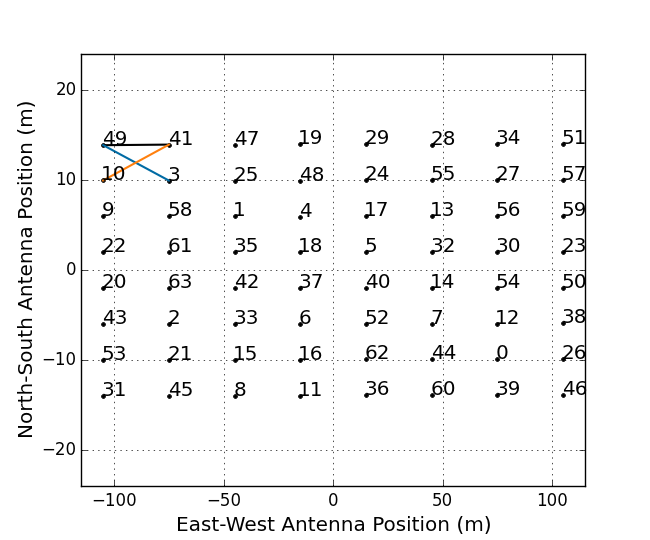
\includegraphics[width=\columnwidth]{plots/antenna_positions.png}
\caption{
Antenna position within the PAPER-64 array.
This analysis only makes use of
east-west baselines between adjacent columns that have row
separations of zero (e.g. 49-41, 41-47, 10-3, \dots)
one in the northward direction (e.g. 10-41, 3-47, 9-3, \dots) or
one in the southward direction (e.g. 49-3, 41-25, 10-58, \dots).
Because of their high levels of redundancy, 
these baselines constitute the bulk of the array's sensitivity for power
spectrum analysis.}
\label{fig:antenna_positions}
\end{figure}

\begin{figure*}
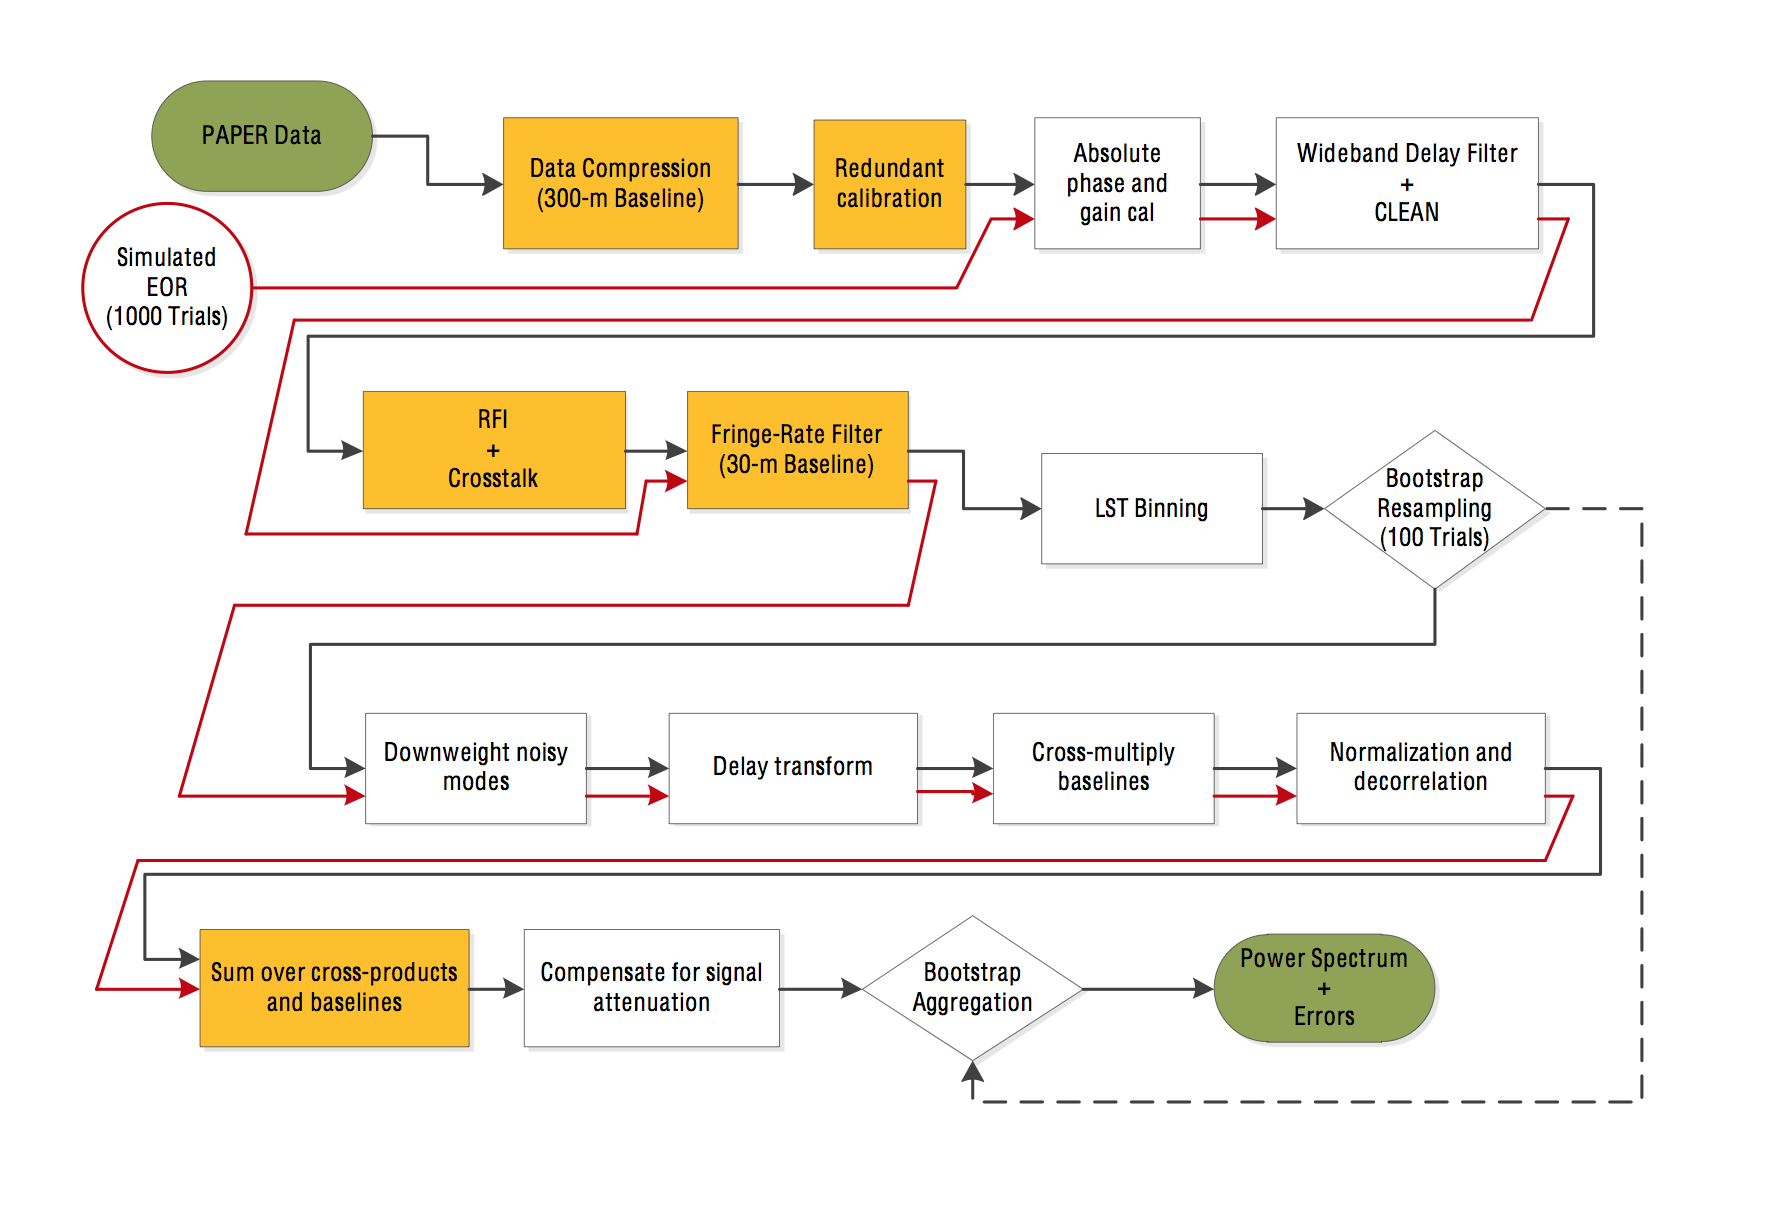
\includegraphics[width=2\columnwidth]{plots/data_flow_chart.png}
\caption
{
The stages of power-spectrum analysis. Black lines indicate data flow; red lines indicate
Monte Carlo simulations used to 
measure signal loss. Yellow boxes indicate stages without associated signal loss.
}
\label{fig:flowchart}
\end{figure*}

We base our analysis on drift-scan observations 
with 64 dual-polarization PAPER antennas (hereafter, ``PAPER-64") deployed 
at the Square Kilometer Array South Africa
(SKA-SA) reserve in the Karoo desert in South Africa
(30:43:17.5$^\circ$ S, 21:25:41.8$^\circ$ E).
Each PAPER element features a crossed-dipole design measuring two
linear (X,Y) polarizations.
The design of the PAPER element, 
which features spectrally and spatially smooth responses 
down to the horizon with a full-width half-maximum of $60^{\circ}$, is summarized in \citet{parsons_et_al2010}
and \citet{pober_et_al2012}.  
For this analysis, we use only the XX and YY polarization cross-products.

As shown in Figure \ref{fig:antenna_positions}, PAPER-64 employs
a highly redundant antenna layout where multiple baselines measure
the same Fourier mode on the sky (P12a; P14).
We rely on all 2016 baselines for calibration,
but only use a subset of the baselines for the power spectrum
analysis. This subset consists of three types of baselines: the 30-m
strictly east-west baselines between adjacent columns (e.g. 41-47
in Figure \ref{fig:antenna_positions}; hereafter referred to 
as {\it fiducial baselines}), 30-m east-west baselines
whose eastern element is staggered one row up (e.g. 10-41), and
those whose easter element is one row down (e.g. 10-58).
We define a redundant group of
baselines as being the set of baselines that have the same grid spacing;
baselines in each
of the three redundant groups described above are instantaneously redundant and
therefore measure the same Fourier modes on the sky. Thus, within a redundant group,
measurements from baselines may be 
coherently added to build power-spectrum sensitivity as $N$ rather than
$\sqrt{N}$, where $N$ is the number of baselines added.  

PAPER-64 conducted nighttime observations over a 135 day period 
from 2012 November 8 (JD 2456240) to 2013 March 23 (JD 2456375). 
Since solar time drifts with respect to sidereal time, this observing campaign
yielded more samples of certain LSTs (and hence, sky positions) than others. 
For the power spectrum analysis, we use observations between 0:00 and 8:30 hours
local sidereal time (LST).  This range corresponds to
a ``cold patch" of sky away from the galactic center where galactic synchrotron power is minimal,
but also accounts for the weighting of coverage in LST.
Figure \ref{fig:coverage} shows our observing field with the contours labeling
the beam weighted observing time relative to the peak, directly over head the
array.

The PAPER-64 correlator processes a 100--200 MHz bandwidth, first
channelizing the band into 1024 channels of width 97.6 kHz, and then
cross multiplying every antenna and polarization with one another for a total of
8256 cross products, including auto correlations.  Following the architecture 
in \citet{parsons_et_al2008}, this
correlator is based on CASPER\footnote{\url{http://casper.berkeley.edu}} open-source
hardware and signal processing libraries \citep{parsons_et_al2006}.  
Sixteen ROACH boards each hosting eight 8-bit analog-to-digital
converters digitize and channelize antenna inputs. New to this correlator,
the cross multiplication engine is implemented on eight servers each receiving
channelized data over two 10-Gb Ethernet links.  Each server hosts
two NVIDIA GeForce 580 GPUs running the open-source cross-correlation code developed
by \citet{clark_et_al2013}.
Visibilities are integrated for 10.7 s on the GPUs before
being written to disk.  All polarization cross-products are saved, although the
work presented here only made use of the XX and YY polarization products.

\begin{figure*}\centering
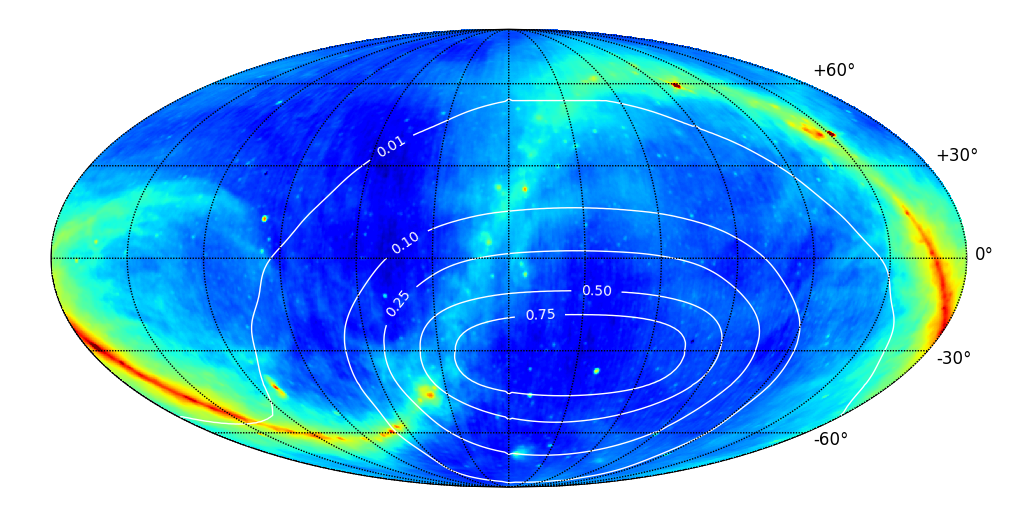
\includegraphics[width=2\columnwidth]{plots/coverage.png}
\caption{The Global Sky Model \citep{deoliveira2008}, illustrating foregrounds to the 21cm
cosmological signal, with 
contours indicating beam-weighted observing time (relative to peak) for the PAPER observations
described in Section \ref{sec:observations}.  The map is centered at 6 hours in right ascension.
}\label{fig:coverage}
\end{figure*}


%%%%%%%%%%%%%%%%%%%%%%%%%%%%%%%%%%%%%%%%%%%%%%%%%%%%%%%%%%%%%%%%%%%%%%%%%%%%%%%%
\section{Calibration}\label{sec:calib}

Foreground contamination and signal sensitivity represent the two major concerns for 21~cm
experiments targeting power spectrum measurements. Sources of foregrounds include
galactic synchrotron radiation, supernova remnants, and extragalactic radio sources.
In the low-frequency radio band (50--200 MHz) where 21~cm reionization
experiments operate, emission from these foregrounds is brighter than the
predicted reionization signal by several orders of magnitude
\citep{ghosh_et_al2011,bernardi_et_al2010,bernardi_et_al2009,ali_et_al2008,deoliveira2008,jelic_et_al2008,santos_et_al2005}.
However, the brightest foregrounds are spectrally smooth, and this provides an
important hook for their isolation and removal
\citep{liu_tegmark2012,petrovic_oh2011,liu_et_al2009}.  Unfortunately,
interferometers, which are inherently chromatic
instruments, interact with spectrally smooth foregrounds to produce unsmooth features that
imitate line-of-sight Fourier modes over cosmological volumes (P12b; \citealt{bowman_et_al2009,morales_et_al2006a}).
One approach to solving this problem involves an ambitious calibration and modeling approach to spatially localize and
remove foreground contaminants \citep{chapman_et_al2013,sullivan_et_al2012,harker_et_al2009,liu_et_al2008,bowman_et_al2008}.
Perhaps the most impressive example of this approach is being undertaken by LOFAR, where dynamic ranges of 4.7 
orders of magnitude have
been achieved in synthesis images \citep{yatawatta_et_al2013}, although it is expected that additional
suppression of smooth-spectrum foreground emission will be necessary \citep{chapman_et_al2013}.

The analysis for this paper employs a contrasting
approach based on the fact that the chromaticity of an interferometer
is fundamentally related to the length of an interferometric baseline.  This relationship, known
colloquially as ``the wedge", was 
derived analytically (P12b; \citealt{vedantham_et_al2012}), and has been confirmed in 
simulations \citep{datta_et_al2010,hazelton_et_al2013} and observationally
\citep{pober_et_al2013,dillon_et_al2013b}.  As described in P12b, the wedge is the result of the delay
between when a wavefront originating from foreground emission
arrives at the two antennas in a baseline.  The fact that this delay is bounded by the light-crossing
time between two antennas (which we call the ``horizon limit'' since such a wavefront would have to 
originate from the horizon) places a fundamental bound on the chromaticity of
an interferometric baseline.  So far, PAPER has had the most success in exploiting this bound
(P14; \citealt{jacobs_et_al2014}). 
%although it is in the process of being applied to MWA observations \citep{nitya}.  
In this analysis, we continue to use the properties of the 
wedge in order to isolate and remove smooth
spectrum foregrounds.

As illustrated in Figure \ref{fig:flowchart},
our analysis pipeline begins by running a compression
algorithm to reduce the volume of our raw data by a factor of 70
(see Appendix A of P14). 
We then calibrate in two stages, which we describe in more detail below.  
The first step uses instantaneous redundancy to solve for the majority of the 
per-antenna internal degrees of freedom in the array.  Second, standard self-calibration is used 
to solve for a smaller number of
absolute phase and gain parameters that cannot be solved by redundancy alone. 
% XXX check if these statements are needed
%After suppressing foregrounds with a
%wide-band delay filter, we average the data in local sidereal time and apply a
%fringe-rate filter to optimally combine the time domain data. 
%These calibratedFinally, we use an
%optimal quadratic estimator to make our estimate of the 21 cm power spectrum.

\subsection{Relative Calibration}
%    -Principles of redundant calibration. Fact that there is no signal loss in
%       this kind of measurement.
%       --PAPER has a redundant configuration. Therefore the number of baselines
%         is larger than the number of unique baselines in the array. There are
%         multiple baselines that measure the same sky.
%       --Introduce uniqe baseline. We define a unique baseline to be the set of
%         redundant baselines of a unique orientation.
%       --All baselines of a unique baseline measure the same sky and
%         therefore, differences between them are what need to be calibrated
%         out. These are the gain variations imparted on the incoming signal by
%         the antenna.
%       --There is no signal loss in this method. Sky signal is the same for
%         each of the redundant baselines is the same and hence any algorithm that
%         preserves common mode signal (which is what redcal does) is necessarily
%         lossless. This is an important point!  
%       --In addtion, because gains are normalized to have a unity magnitude the
%         input arn output flux scale are the same. (This is an omnical thing)
%         
%    -What can we solve for and what can't we solve for. We can solve for the
%     relative complex gains between antennas, but not the absolute gain and phase.
%       --Because redundant calibration does not fold in any outside
%         information about the sky that we are observing, it inherently is a
%         relative calibration scheme that solves for the relative gains and
%         phases of antennas within the array. 
%       --Therefore, we cannot solve for the absolute phase and gain of the
%         array. There is not enough information.
%       --Absoulte phase and gain calibration are addressed in later sections.
%

The grid-based configuration of PAPER antennas allows a large number of antenna
calibration parameters to be solved for on the basis of redundancy (P14; P12a;
\citealt{zheng_et_al2014}).  Multiple baselines of the same length and
orientation measure the same sky signal. Differences between redundant
baselines result from differences in the signal chain, including amplitude and
phase effects attributable to antennas, cables, and receivers.  Redundant
calibration only constrains the relative complex gains between antennas and is
independent of the sky. Since redundant calibration preserves signals common to
all redundant baselines, this type of calibration is lossless. 

%    -Summary of the procedure of redundant calibration. This should be mixed in
%     with the equations from Zheng et. al.
%       --Two flavors of redundant calibration : logcal and lincal. Cite
%         liu,zheng.
%       --logcal takes log of equation 3 in zheng et. al., and thus becomes a
%         linear system. Can then solve for the log of the antenna gains, as
%         well as the true visibility of the sky as measured from a unique
%         baseline. 
%       --lincal is the linearization via taylor expansion of the same equation
%         3. This provides us with a better solution. The reason for doing
%         lincal is that logcal is a biased estimator. 
%       --Because there are more baselines than the number of unique baselines, 
%         we have an overdetermined system of equations and therefore can
%         uniquely solve for all of the gains and "true" visibilities.

In practice, redundant calibration often takes on two flavors: log calibration (LOGCAL) and
linear calibration (LINCAL) \citep{liu_et_al2010,zheng_et_al2014}. LOGCAL uses 
logarithms applied to visibilities (equation 4 of
\citealt{zheng_et_al2014}) to give a linearized system of equations
\begin{equation}\label{eqn:logcal}
    \log{v_{ij}} = \log{g_{i}^{*}} + \log{g_{j}} + \log{y_{i-j}},
\end{equation}
where $g$ denotes the 
complex gain of antennas indexed by $i$ and $j$, and $y$ represents the ``true" visibility 
measured by all redundant baselines.  In solving for per-antenna gain parameters with
a number of measurements that scales quadratically with antenna number, redundancy gives 
an over-constrained
system of equations that can be solved
using traditional linear algebra techniques.
While LOGCAL is useful for arriving at a coarse solution from initial estimates that are far
from the true value, LOGCAL has the shortcoming of being a biased by the asymmetric behavior
of additive noise in the logarithm \citep{liu_et_al2010}.

LINCAL, on the other hand, uses a Taylor expansion of the visibility around initial
estimates of the gains and visibilities, 
\begin{equation}\label{eqn:lincal}
v_{ij} = g_{i}^{0*}g_{j}^{0}y_{i-j}^{0} + g_{i}^{1*}g_{j}^{0}y_{i-j}^{0} +
         g_{i}^{0*}g_{j}^{1}y_{i-j}^{0}+g_{i}^{0*}g_{j}^{0}y_{i-j}^{1},
\end{equation}
where $0$ denotes initial estimates and $1$ denotes 
solutions we fit for.  Using initial
estimates taken from LOGCAL, LINCAL constructs an unbiased estimator.

%    -How was this calibration applied to the data. 
%       --Using omnical package. Give credit jeff and url to omnical. Cite
%         paper.
%       --Implements both logcal and lincal. Discuss the speed ups. 
%       --gains were applied to the uv datasets and written out in the same
%         format. However, Omnical is quite general and solutions can be written
%         out in text files and adapted to other file formats.
%    
%    -Removing additive offset and what is the time cadence of all of this.
%       
%    -Diagnostic figures : Chi-squared, complex plane, stability vs. time and
%                          frequency.

Implementation of redundant calibration was done with the 
OMNICAL\footnote{https://github.com/jeffzhen/omnical}
package, an open-source redundant calibration package
\citep{zheng_et_al2014}. This
package implements both LOGCAL and LINCAL, solving for a complex gain solution
per antenna, frequency, and integration. The per integration solutions are then
applied to visibilities and the results are shown in \ref{fig:omniview}.

\begin{figure*}
\centering
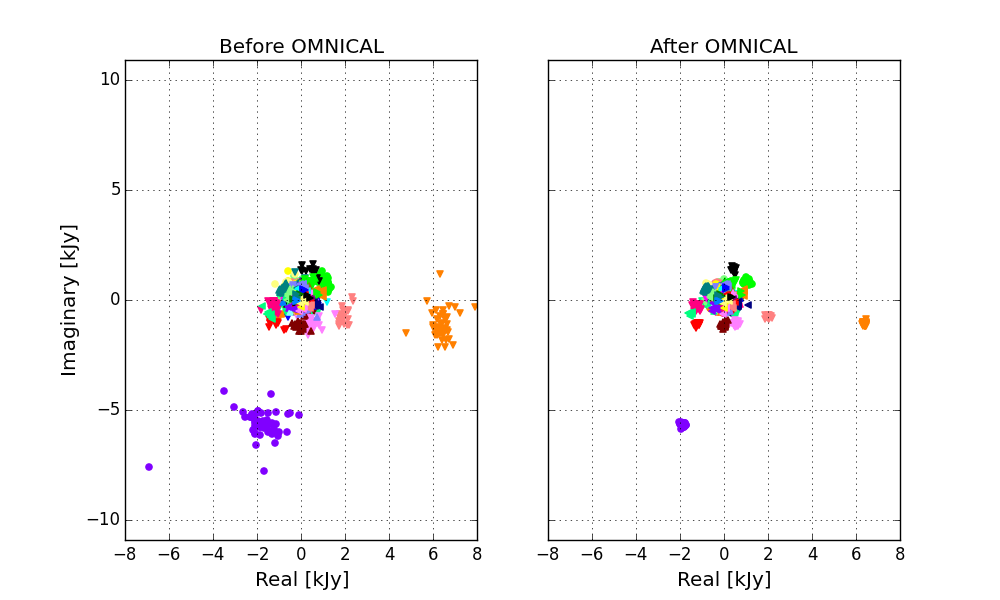
\includegraphics[width=1.5\columnwidth]{plots/omniview_64.png}
\caption{
PAPER visibilities plotted in the complex plane before (left) and after (right)
the application of redundancy-based calibration with OMNICAL \citep{zheng_et_al2014}.
All baselines in the array measured at 159 MHz for a single time integration are plotted.
Instantaneously redundant baselines are assigned the same symbol/color.
The tighter clustering of redundant measurements with OMNICAL indicates improved
calibration.
} \label{fig:omniview}
\end{figure*}

\begin{figure}
\centering
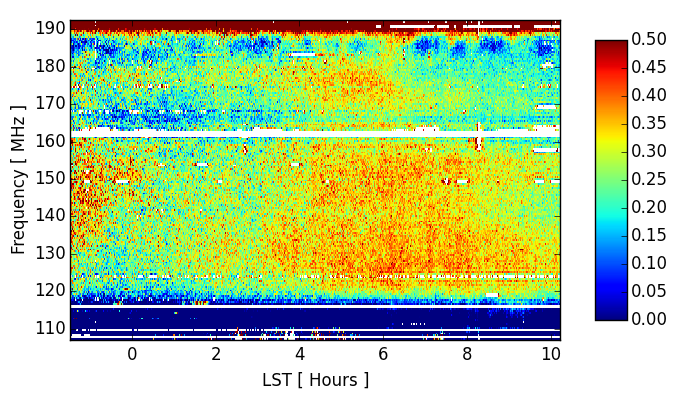
\includegraphics[width=\columnwidth]{plots/chi2.png}
\caption{
Log of $\chi^{2}$ of all baseline residuals after the application of OMNICAL.
The plot comprises a observations over one day, with a frequency resolution of
492 kHz and a time resolution of 42.9 s.
} \label{fig:chi2}
\end{figure}

In addition to solving for gain solutions, OMNICAL also characterizes the
quality of the calibration parameters by calculating the $\chi^{2}$ for every
integration. As defined in \cite{zheng_et_al2014}, 
\begin{equation}\label{eqn:chi2}
    \chi^{2} = \sum_{ij}\frac{|v_{ij} - y_{i-j}g^{\ast}_{i}g_{j}|^{2}}{\sigma^{2}_{ij}},
\end{equation}
where $\sigma^{2}$ is the noise in the variance of the visibility. The $\chi^{2}$
measures the deviation of measured visibilities to that of the best fit model
derived from the LINCAL, and gives us a tool to use in order to check the
quality of our data, with large $\chi^{2}$ corresponding to a bad fit. Figure
\ref{fig:chi2} shows the $\chi^{2}$ for all frequencies for and entire day. The
noise model used was the variance of the visibilities for a given frequency and
LST bin. The $\chi^{2}$ can be a metric used for RFI flagging and removal because
when RFI dominates, at a given frequency or time, the measured visibility would
be considered a poor fit to the model. This data set did not use the $\chi^{2}$
as a metric but preliminary studies have shown it's efficacy on PAPER-128
observations.

[XXX need to talk about the additive offset removal from visibilities and
solutions.]

\subsection{Absolute Calibration} 
%    -Selfcal to pictor, fornax, and crab (to get the north-south components).
%       --Reiterate that redundant cal does not solve for the overall flux and
%         phase parameters. 
%       --There are two final phase parameters we must solve
%         for in order to correctly phase to a source on the sky. Redundancy
%         only gets you so far, but still need to be able to unambiguously phase
%         to sources.
%       --We use self calibration to solve for the global phase parameters using
%         Pictor A, Fornax A, and Crab Nebula. 
%       --
%
%    -Diagnostic Plots: Show Field image from Bernardi. This will give
%     confidence in a good absolute phase calibration.

After solving for the relative complex gains of the antennas using redundant
calibration, an overall phase and gain calibration remains unknown. We use the
standard self calibration method for radio interferometers to solve for the
absolute phase calibration. We used Pictor A, Fornax A, and the Crab Nebula to
fit for the overall phase solutions. Figure \ref{fig:field_image} shows an image
of the field with Pictor A (5:19:49.70, -45:46:45.0)  and Fornax A
(3:22:41.70,-37:12:30.0).
%The measured source positions are the same as the catalogue positions for these sources.

%    -Calibrated to Pictor A. 
%       --As before, redundant calibration cannot set a global flux scale. For
%       our measurements to be correct, we need to set a fluxscale. We use
%       Pictor A to set our fluxscale. Cite Dannys pictor paper.
%      
%    -Our bandpass model is a 9th degree polynomial. 
%       --In order to set our fluxscale, we beamform our data upto pictor A,
%         summing baselines, and then then fit a 9th degree polynomial to the
%         bandpass. This is our measure of the spectrum of Pictor A. 
%       --Because we are beamforming to pictor and fitting a polynomial to the
%         bandpass, there is signal loss. This signal loss is of the 
%    -Tabulate signal loss due to this model. Averaging over Nbls, times gives us
%     an average over independent uv modes.
%       --Working on this... a few questions about it.
%
%    -The actual signal loss on a given mode is L/N where L is the loss for a
%     single instance of the beamform (one time, one baseline) and N is the
%     number of baseline and times that were summed.
%
%    -PLOTS: 
%        --A plot that is the phased to pictor beamform gain 
%          (or maybe just a single channel for all days.
%        --The measured and theoretical pictor spectrum 
%        --A comparison to the PSA32 Flux CAL.

We then set our over all flux scale by using Pictor A as our calibrator source
with source spectra derived in \cite{jacobs_et_al2013}, 
\begin{equation}
    S_{\nu} = S_{150}\times\left(\frac{\nu}{150MHz}\right)^{\alpha},
\end{equation}
where $S_{150} = 382~\text{Jy} \pm 5.4$ and $\alpha = -.76 \pm .01$, with
1$\sigma$ error bars.


%To derive the source spectrum from our measurements, we use lst averaged data (see
%section \ref{sec:lstbin}) containing foregrounds for the hour before and after from
%where Pictor A transits. We image, in 15 minute snapshots for this data set,
%every frequency channel. The source spectra is derived per snapshot and we average
%these together, weighting by the primary beam in the direction of Pic A to get
%the measured spectrum of Pictor A. To fit our bandpass, we divide the model
%spectrum with ourAmeasured spectrum and fit a ninth-order polynomial over a
%frequency range from 120-170MHz. Figure \ref{fig:pic_spec} shows the derived
%Pictor A spectrum and the model spectrum derived from \cite{jacobs_et_al2013}.

To derive the source spectrum from our measurements, we use data that have been
LST-averaged prior to the wide-band delay filter described in Section
\ref{sec:wbd_filtering}, for the hour before and after the transit of Pictor A.
We image a $30^\circ \times 30^\circ$ field of view for every frequency channel
for each 10 minute snapshot and apply uniform weights to the gridded
visibilities. We account for the required three dimensional Fourier transform in
wide field imaging by using the w-stacking algorithm implemented in WSclean
\citep{offringa_et_al2014} – although we note that the standard w-projection
algorithm implemented in CASA\footnote{http://casa.nrao.edu} gives similar
performances as the PAPER array is essentially instantaneously coplanar.  A
source spectrum is derived for each snapshot by fitting a two dimensional
Gaussian to Pictor A by using the
PyBDSM\footnote{http://www.lofar.org/wiki/doku.php?id=public:user\_software:pybdsm}
source extractor. Spectra are optimally averaged together by weighting them with
the primary beam model evaluated in the direction of Pictor A. To fit our
bandpass, we divide the model spectrum by the measured one and fit a 9-th order
polynomial over the 120-170 MHz frequency range. Figure \ref{fig:pic_spec} shows
the calibrated Pictor A spectrum and the model spectrum from
\cite{jacobs_et_al2013}.

\begin{figure}
\centering
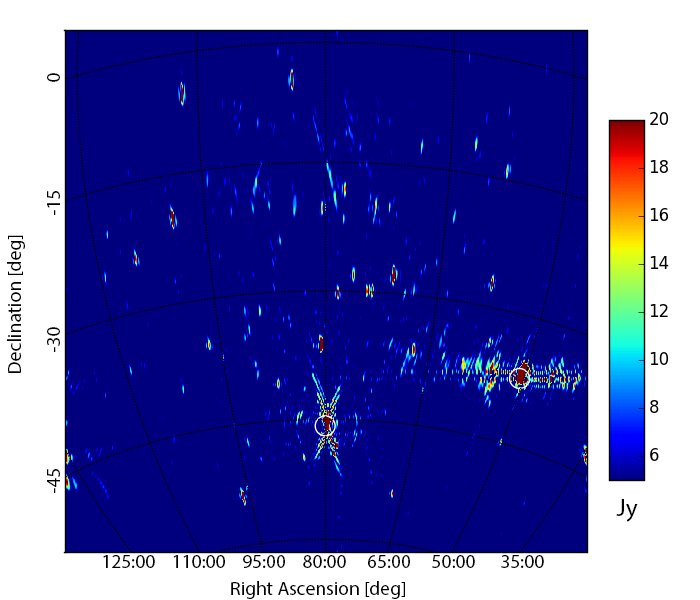
\includegraphics[width=\columnwidth]{plots/picimg_cs.png}
\caption{
PAPER-64 image of a field including Pictor A and Fornax A, with black circles
indicating catalog positions \citep{jacobs_et_al2011}. Image was synthesized with two hours
of visibilities while Pictor A was in transit and 53 MHz of instantaneous
bandwidth from 120 to 173 MHz.  Image quality is limited by the redundant
configuration of the array (e.g. grating lobes as a result of periodic antenna
spacing, elongated lobes arising from poor uv-coverage in the north-south
direction).  Nonetheless, this image demonstrates accurate phase calibration
over a wide field of view.
} \label{fig:field_image}
\end{figure}


\begin{figure}
\centering
%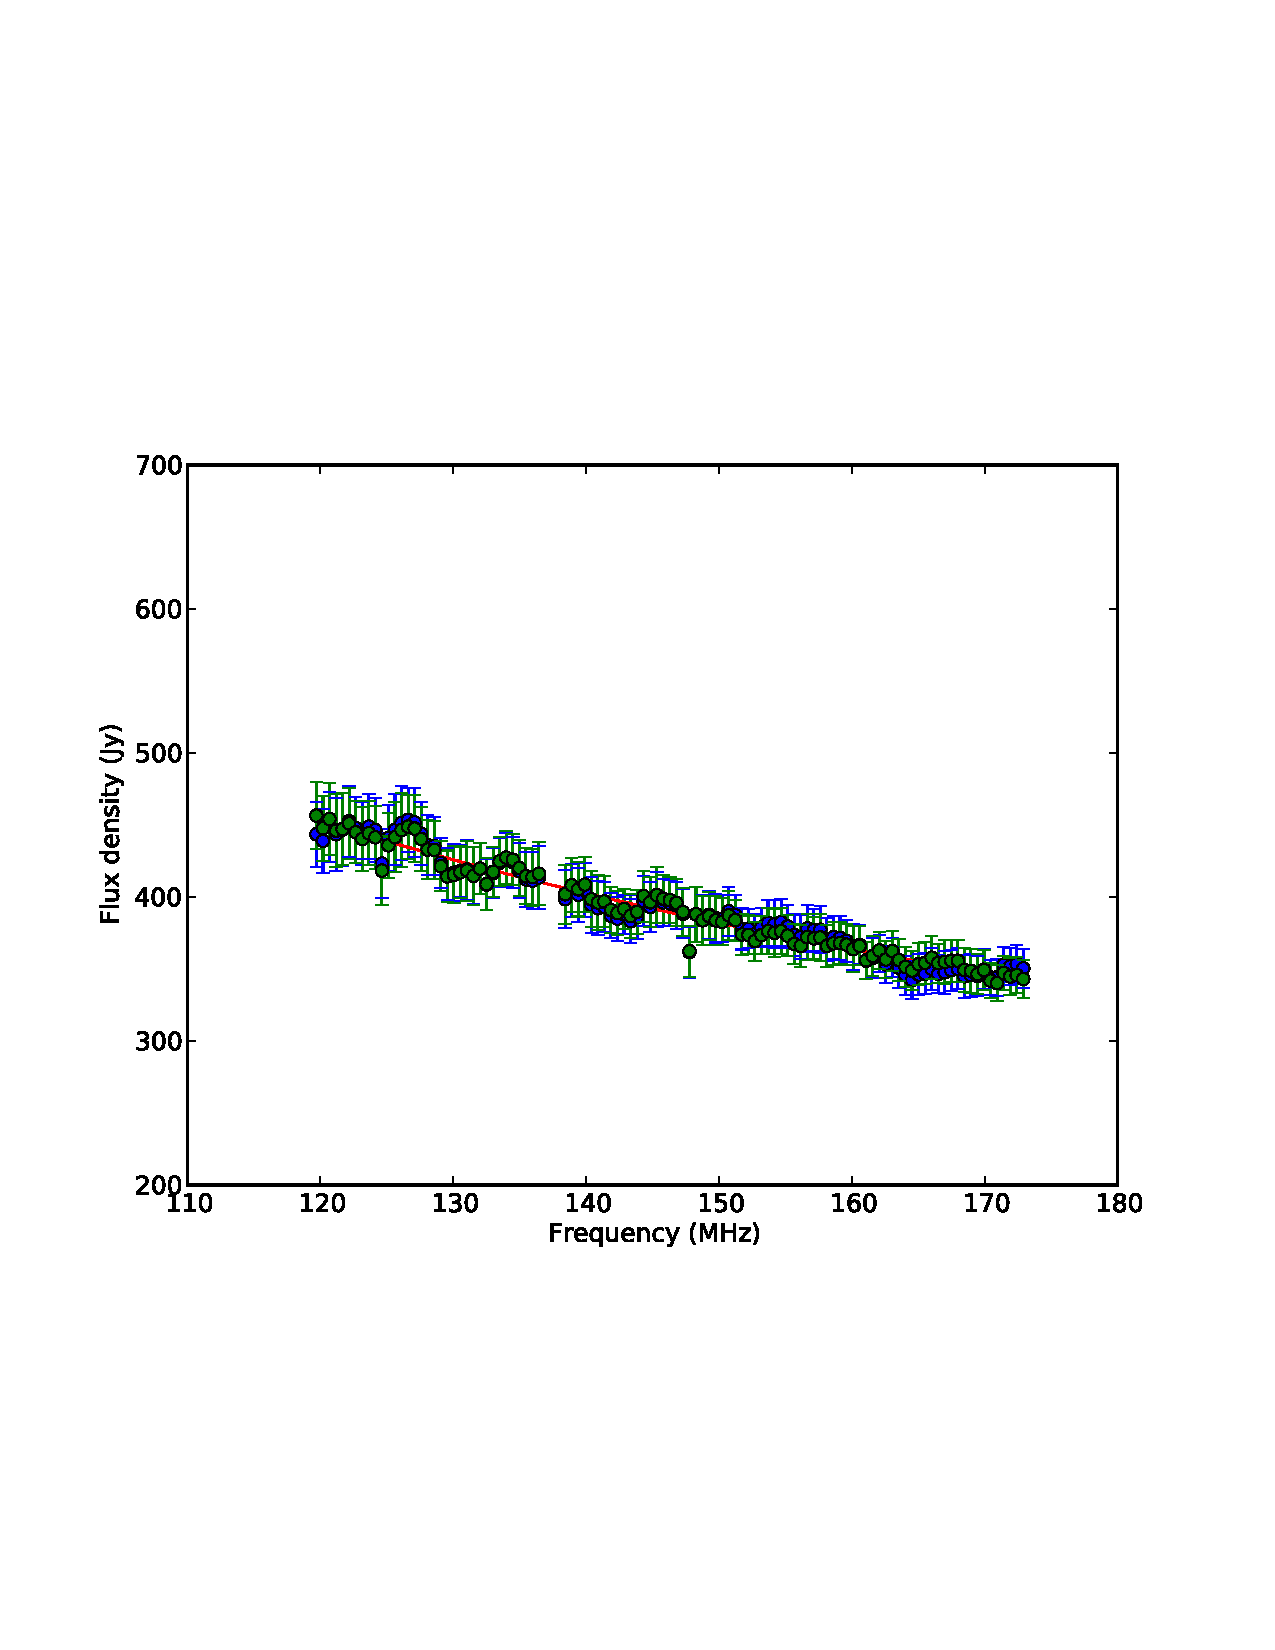
\includegraphics[width=\columnwidth]{plots/PicA_normalized_spectrum.pdf}
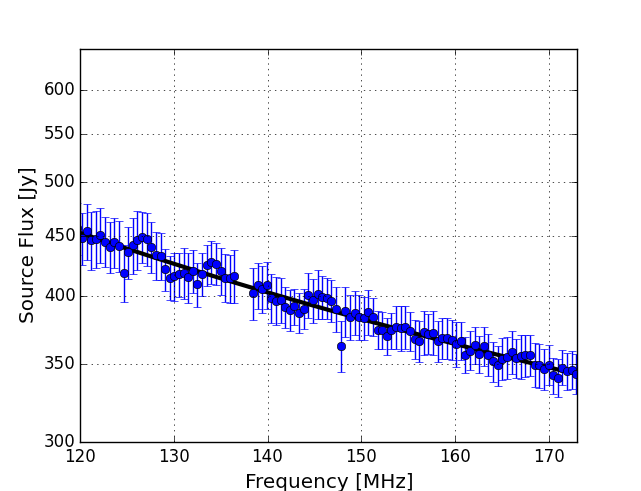
\includegraphics[width=\columnwidth]{plots/picspec.png}
\caption{
Measured spectrum of Pictor A in Stokes I (blue) relative to its catalog
value (black; \citealt{jacobs_et_al2013}).  Flux measurements are
extracted from images of Pictor A, made independently for each frequency channel in
10 minutes snapshots as Pictor transits between hour angles of -1:49
and 1:10.  Each measurement is then divided by the PAPER beam model and
averaged to obtain the measured spectrum, which serves to characterize the flux
scale of the PAPER-64 observations. Error bars indicate 68\% confidence
intervals, derived from the Gaussian fits in the source extractor used in
measure the flux in PyBDSM.
[XXX How are these errors averaged? Did you use the same beam weighting?]
}\label{fig:pic_spec}
\end{figure}

[XXX ZSA take a look at this paragraph]
Fitting a polynomial to the bandpass has the potential for signal loss which
would include suppressing mode due to the cosmological signal. In order to
quantify the signal loss associated with fitting a ninth degree polynomial to
the bandpass, we run a Monte Carlo simulation of the effect the bandpass has on
a model 21-cm reionization signal. We construct a model baseline visibility as a Gaussian
random signal with $\mu=0$ and $\sigma=1$ offset by 5 orders of magnitude
multiplied by the derived bandpass for every independent mode measured.  We
calculate the total number of independent modes by counting the number of
independent uv-modes sampled for the different baseline types and the two hour
time interval used to measure the bandpass. We average each mode together and
fit a 9th degree polynomial and using that as our measured bandpass in this
simulation.  Finally, to measure the lost power as function of
$k$-mode, we compare the power spectra from the output of the simulated
signal to the input amplitude in and find that between $-0.06 < k < 0.06$, the
signal loss is less than $3\%$ and at the mode right outside the horizon is
$.0000002\%$. The signal loss decreases for higher $k$'s.


%These lists were My bullet points.
%\begin{itemize}
%    \item{Overview of the calibration with emphasis on Omnical.}
%    \item{Rough Calibration : Can cite Parsons 2014 for the details.}
%    \begin{itemize}
%        \item{Discuss the first pass of redundant phase and gain calibration.
%              Absolute phase calibration using pictor, fornax and crab in the
%              fit.}
%        \item{Absolute flux scale using Pictor A. Want to address signal loss.
%             Maybe delay the issue of signal loss to a "Signal Loss" section
%             which takes into account the signal loss in various stages of the 
%             analysis?}
%        \item{Add in details of the loss of eor signal. Do simulations to get
%              numbers. }
%        \item{Plots : Measured pictor spectrum with comparison to the Danny
%              pictor spectrum. Maybe some simulation plots showing the signal
%              loss due to the polynomial fit to pic spec.}
%    \end{itemize}
%    \item{Omnical}
%    \begin{itemize}
%        \item{What is omnical?}
%        \item{Why are we using it? To get a frequency/time dependent
%calibration. Need to address why this is not overfitting. That is why is this
%just not flatting everything out.}
%        \item{Address non-possibility of signal loss.}
%        \item{Refresh formalism (do this here or in the intro of calibration?)}
%        \item{What is it doing? logcal/lincal. Chi-squared and how that
%              determines the goodness of the fits to the model baselines. What
%model are we using? Is it a good model?}
%        \item{Plots: Chi-squared plots. Compex plane plots that show
%              improvements over uncalibrated/rough/omnical calibrated. 
%              Time and frequency stability.}
%    phase to pic gain, pic spec, comparison to psa32.
%    \end{itemize} 
%\end{itemize}

%OLD TEXT START
%\subsubsection{Overview}
%As the name suggests, redundant calibration (\cite{liu_et_al2010},
%\cite{zheng_et_al2014}) uses redundancy within the array to solve for relative
%phases and gains of the antennas. To explain redundant calibration, suppose that
%the baseline between antennas $i,j$ measure a visibility $v_{ij}$, then we have 
%
%\begin{equation}\label{eqn:redcal}
%    v_{ij} = g_{i}g_{j}^{*}y_{i-j} + n_{ij},   
%\end{equation}
%where $g_{i}$,$g_{j}$ are the complex gains due to antenna $i$ and antenna $j$,
%respectively, $y_{i-j}$ is the true visibility measured by perfect antennas
%$i$,$j$ for the given baseline type, and $n_{ij}$ is the residual noise from
%the baseline.  If the number of baselines of a given type is much greater than
%the number of baselines types this problem is over constrained and $g_{i}i$,
%$g_{j}$, and $y_{i-j}$ can be solved for. PAPER is in this limit due to the
%maximally redundant configuration as shown in figure \ref{fig:antenna_pos}. 
%
%Redundant calibration comes in two flavors: log calibration and linear
%calibration. Log calibration, or logcal for short, takes the logarithm of
%equation \ref{eqn:redcal} to give a linearized system. Hence, solutions can be
%solved for by using standard linear algebra techniques. However, this method is
%biased. On the other hand linear calibration, or lincal for short, is an
%unbiased method of solving for the complex gain solutions. In this method
%equation \ref{eqn:redcal} is Taylor expanded about an initial guess for the
%$g_{i}$'s and $y_{i-j}$'s to give a linearized equation which can be used to
%solve for the complex gains and sky model. 
%
%In this analysis we used a logcal algorithm based in delay space to get a rough
%calibration of the dataset. This was followed by an absolute calibration to set
%the overall phase and flux scale using a self calibration. We used model phase
%centers of Pictor, Fornax A, and Crab Nebula. The absolute amplitude is set
%by the flux of Pictor A found in \cite{jacobs_et_al2013}, whose spectrum is
%defined by 
%\begin{equation}
%    S_{\nu} = 382(\frac{\nu}{150 MHz})^{-.76} Jy.
%\end{equation}
%
%Finally, we used the Omnical calibration package to do another round of
%redundant calibration to get even more accurate calibration parameters.
%
%\subsection{logcal-for lack of a better title}
%We first perform the same calibration that was
%done in \citep{parsons_et_al2014a}. That is, we use redundancy to do a relative
%phase\footnote{In actuality, we solve for delays to get around phase wrapping
%issues. These delays are applied to visibilities as $e^{2\pi{i}\tau\nu}$}
%calibration between antennas, which removes the electrical delays from cables in
%the signal path. Due to redundancy, we can calibrate out all of the per-antennas
%delays in the signal path relative to two delay parameters which we call
%$\tau_{ns}$ and $\tau_{es}$. These delays are the relative electrical delays
%that correspond to baseline delays in the north-south and east-west component
%for 2 reference baselines (49-10 and 49-41,respectively). These solutions were
%then applied to the data set which was calibrated again with Omnical. 
%
%The application of this calibration to the data set before Omnical was needed
%because in order to calibrate accurately, Omnical needs to have a rough estimate
%for the calibration solutions for every antenna. In \cite{zheng_et_al2014}, a
%model of the sky was used in order get the rough estimate of the solutions.
%Here, we use actual sky data to get the rough calibration. Because the solutions
%are derived from the instrument, we can incorporate into the solutions antenna
%based variations. 
% 
%The antenna based
%delay solutions vary as much as a couple nanoseconds day to day when solutions
%are averaged over hour long timescales withing a day. However, the variations in
%solutions is worse when only averaging over ten minute time scales. Therefore
%need for better calibration is requred.  We use self calibration to derive the
%two unknow parameters, $\tau_{ns}$ and $\tau_{ew}$, by using the Crab Nebula,
%Fornax A, and Pictor A.
%
%Note that there is no possibility of signal loss (see \citep{parsons_et_al2014a}).
%
%\subsection{Gain Calibration}
%Gain calibration was derived on the basis of redundancy and self calibration.
%The phase calibrations described above, simultaneously also calibrated for the
%relative gain variation between antennas. Again we can only calibrate to a fiducial
%antenna (49) whose gain is defined as unity. We then perform a self calibration
%to set the flux scale to Pictor A whose spectrum is derived in
%\citep{jacobs_et_al2013}. We use the same methods describes in \citep{parsons_et_al2014a}.
%
%Figure \ref{fig:bmfom_pic} shows that dataset beamformed to Pictor A, with log
%janskies on the y axis and lst on the xaxis for a frequncy of .1 + (120/203)*.1/203. 
%As can be seen, the day to day variation in the formed beam has a fractional
%spread of about 10$\%$.  This shows the stability of the instrument and the well
%behaved calibration solutions derived above. 
%
%\subsection{Omnical}
%(How did we know that our calibrations were not good enough? Because of the power
%spectrum? PSA32? We did beamform data to pictorA and say that vs LST, the
%beamform matched well day to day with a fractional spread of about 10$\%$) 
%
%The complex gain solutions found in the previous calibration pipeline were
%averaged together in time and one solution per frequency was used for the array.
%This jived with the philosophy that the array was stable in time and frequency.
%However, upon further review of this data set, it seemed more and more likely
%that this was not the case anymore. (Is this even true? What specifically? Think
%Man!) 
%
%Due to clues that showed that our data set had time dependent calibration
%solutions, it was imperative that we do a better job at calibrating our array.
%
%The Omnical redundant calibrator
%package\footnote{https://github.com/jeffzhen/omnical} (omnical) performs
%redundant calibration for every time and frequency in a dataset using both
%logcal and lincal methods as described in \cite{zheng_et_al2014}. It also
%contains methods on the quality of the solutions by providin a chi-square for
%the fits to the data. 
%
%For this dataset, omnical first performed a logcal (again) to attain a solution
%per time and frequency. This solution was passed to lincal which iteratively
%solved for the complex gain solutions. The convergence criteria was when the
%$\chi^{2}$ decreased by less than $.01\%$. The $\chi^{2}$ for the fit used in
%Omnical is given by 
%\begin{equation}
%    \chi^{2} = \sum_{ij}|v_{ij} - y_{i-j}g_{i}^{*}g_{j}|^{2},
%\end{equation}
%
%which differs from normal nomenclature because we are not inverse varaince
%weighting. Note that this $\chi^{2}$ is summing over all baselines and hence 
%giving more weight to higher gains. Note that omnical fits for each of the
%complex gains and the model visibility, $y_{i-j}$,  for a unique baseline.
%Using this information, figure \ref{fig:chi_2} shows that the $\chi^{2}$ is close
%to 1 for all channels and time (for this day of data). need noise model for
%this.
%
%Figure \ref{fig:gain_solutions} shows the gain solutions output by omnical. The
%amplitude of the gains are roughly order unity through out. These are relative
%gains between antennas and hence the over flux scale set to Pictor A is still
%valid. The absolute calibration is still valid. 
%
%Since Omnical outputs a model visibility of what a unique baseline should
%measure, which is derived from the data by removing all of the variation between
%unique types of baselines and averaging, we are able to use these outputs as our
%dataset. Infact, this is what is done. 
%%waterfalls of chi squared and solutions.
%%day to day repeatability.
%%The output of the omnical - 
%%
%OLD TEXT END



\subsection{Wideband Delay Filtering}\label{sec:wbd_filtering}
%   -Can cite Parsons 2014a
%       --We use the same wbd filter as in Parsons 2014a. That is we do a per
%         baseline delay filtering with a buffer of 15 nanoseconds. 
%   -Quantify signal loss. 
%       --I think this is the same as before. Since delay filtering is done on a
%       per baseline basis, the signal loss from the previous paper and this one
%       is the same. We are using the same filter.
%   -PLOTS:
%        --waterfalls of before and after cleaning.
%        --signal loss vs. k_parallel


Before implementing our foreground removal techniques, we combine the two
linear polarizations for an estimate of stokes I as per \citet{moore_et_al2013}.
Namely, Stokes I can be estimated as 
\begin{equation}\label{eqn:stokesi}
    V_{\rm I} = \frac12(V_{\rm XX}+V_{\rm YY}),
\end{equation}
where $V_{\rm XX}$ and $V_{\rm YY}$ are the visibilities of the two linear
polarizations measured by the interferometer. There are some important caveats
to the estimate of Stokes I provided by equation \ref{eqn:stokesi}. One
important caveat is that it neglects the beam asymmetry  between the two linear
polarization states. This mismatch can cause polarization leakage from Stokes
Q into Stokes I, thus contaminating  our measurement of the power spectrum with any polarized emission from the sky.
This effect for PAPER, as shown in \citet{moore_et_al2013}, leaks 4\% of Q in to
I.  We offer no correction for this effect, but in turn put some limits on
polarization leakage discussed later. 

Foreground removal techniques discussed in the literature include spectral
polynomial fitting \citep{wang_et_al2006,liu_et_al2009,bowman_et_al2009},
principle component analysis
\citep{paciga_et_al2013,paciga_et_al2011,liu_tegmark2011,masui_et_al2013},
non-parametric subtractions
\citep{harker_et_al2009,chapman_et_al2013}, and inverse
covariance weighting
\citep{dillon_et_al2013b,liu_tegmark2011,dillon_et_al2013a}, and per-baseline delay filtering described in
P12b and \citet{petrovic_oh2011}. The delay spectrum filtering technique is
well suited to the maximum redundancy PAPER configuration which is not
optimized for the other approaches where high fidelity imaging is a
pre-requisite.   The delay spectrum foreground clean method is described in
detail by P14; its application is unchanged here.  In summary; we Fourier
transform each baseline spectrum into the delay domain  


\begin{align}\label{eqn:delay_transform}
\tilde{V}_\tau &= \int{W_\nu A_\nu I_\nu
                   e^{-2\pi{i}\tau_{g}}\cdot e^{2\pi{i}\tau\nu}d\nu} \\\notag
                %&= \int{W_\nu A_\nu I_\nu
                %   e^{-2\pi{i}\nu(\tau_{g}-\tau)}d\nu} \\\notag
                &= \tilde{W}_\tau \ast \tilde{A}_\tau \ast
                   \tilde{I}_\tau \ast
                   \delta(\tau_{g} - \tau),
\end{align}
where $A_\nu$ is the frequency dependent antenna response, $W_\nu$ is a sampling function
that includes RFI flagging and a
Blackman-Harris tapering function that minimizes delay-domain scattering 
from RFI flagging, and $I_\nu$ is the source
spectrum.  In delay domain, a point source appears as a $\delta$-function at
delay $\tau_{g}$, convolved by the Fourier transforms of the
source spectrum, the antenna response, and the
sampling function. We note that the antenna response effectively determines a finite bandpass,
which imposes a lower bound 
of $1/B \approx 10 ns$ on the width of any delay-domain convolving kernel.
As per
\cite{parsons_backer2009} and P14, we deconvolve the kernel
resulting from $W(\tau)$ using an iterative CLEAN procedure
\citep{hogbom1974} restricting CLEAN components to fall within the horizon plus
a 15-ns buffer that includes the bulk of the kernels convolving the $\delta$-function
in equation \ref{eqn:delay_transform}.
To remove the smooth spectrum
foreground emission we subtract the CLEAN components from the original
visibility.

\begin{figure*}
\centering
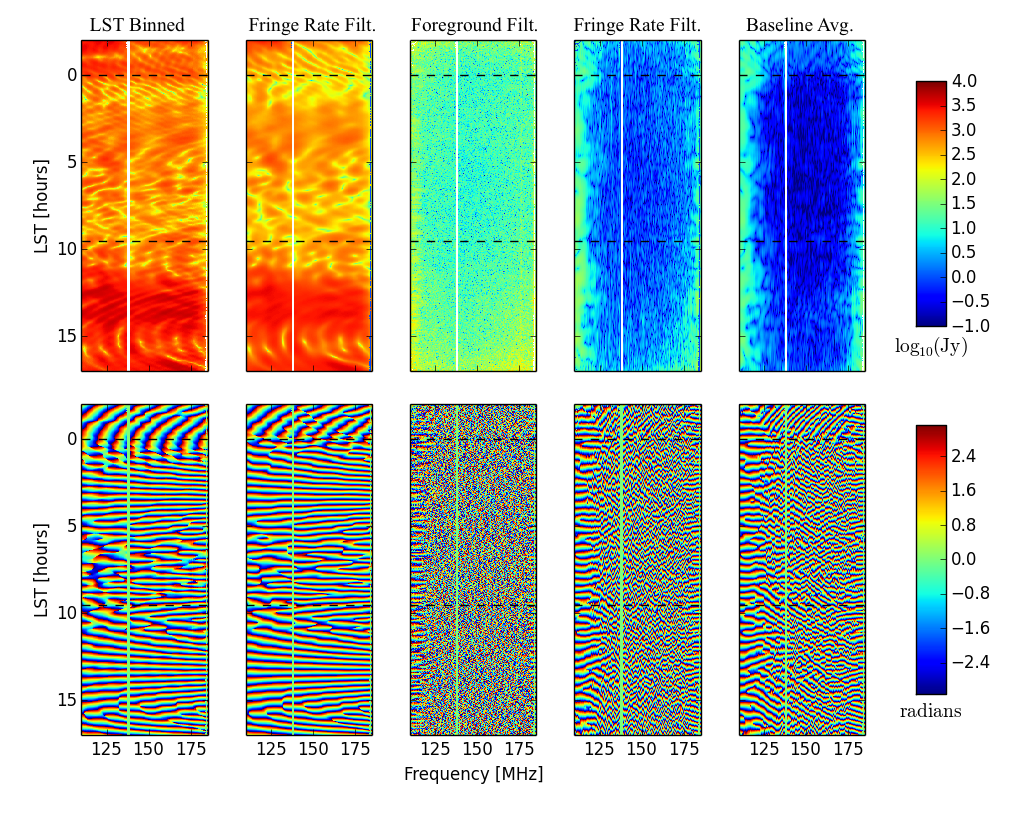
\includegraphics[width=2\columnwidth]{plots/waterfalls_labeled.png}
\caption{
Visibilities measured by a fiducial baseline in the PAPER-64 array, 
averaged over 135 days of observation.  From left to right, columns represent
data that: (1) contain foregrounds prior to the application of a wideband
delay filter or optimal fringe-rate filtering, (2) are fringe-rate filtered but
not delay filtered, (3) are delay filtered at 15 ns beyond the horizon limit but
are not fringe-rate filtered, (4) are both delay and fringe-rate filtered,
and (5) are delay and fringe-rate filtered and have been averaged over all
redundant measurements of this visibility.  The top row shows signal amplitude
on a logarithmic scale; the bottom row illustrates signal phase.
Dashed lines indicate the 0:00 -- 8:30 range in local sidereal time (LST) used for power
spectrum analysis.  Away from the edges of the observing band, over four orders 
of magnitude of foreground suppression is evident.
} \label{fig:waterfalls}
\end{figure*}

Applying the delay filter to fiducial baselines used in the power spectrum analysis,
foregrounds are suppressed by $\sim$4 orders of magnitude in power, or
 -40 dB of foreground suppression, as seen in Figure
\ref{fig:waterfalls}. As discussed in P14, there is a small amount of signal loss
associated with this foreground filter, for the baselines and filter parameters the loss was found to be 4.8\% for the
first mode outside of the horizon, 1.3\% for the next mode out, and less than
.0015\% for the higher modes.  [XXX are we applying these numbers to the pspec or just calling it negligible? The are applied to their corresponding modes.]  

After the wideband delay filter, we remove a second layer of RFI and crosstalk
 which was overshadowed by the foreground signal. RFI are excised with 
 a filter which flags values $3\sigma$ above the median using a variance calculated in a localized time and frequency window.  Cross-talk, which is an overall complex offset to the visibility, due to small couplings between independent analog signal chains, is removed by subtracting a ten minute long average from each baseline. Normally, hour long averages are needed for foreground contained data
to wash out the fringes from the said foregrounds to detect the static 
bias that is crosstalk. With foregrounds removed, we do not have this
complication since bright foregrounds are not dominating the average and are
able to remove the offset by subtracting shorter sums.

The final step is to average the entire season into local sidereal
time (LST) with bins of width 43 seconds, a bin size that matches the fringe-rate filter applied
in the compression step. The full season was 135 days long; of these 124 days were included in the average. 

Sporadic RFI events (i.e. occurring rarely in an entire season) can skew individual LST bins away from the median value of
the sky at a given LST, deviating from Gaussian statistics. To catch these
events, we compute the median of a LST bin for each frequency and flag points  3
$\sigma$ above the median, before averaging. This filter mitigates
the effects of non Gaussianity in time, which is most likely due to spurious
RFI events. The median statistic used here ensures that there is no signal
loss due to this filter. [XXX why is this?]

We make two separate LST-binned data sets, averaging every other julian day
together to obtain an "even" and "odd" dataset. The use of these two data sets
allows us to construct an unbiased power spectrum estimate, as well as running
jackknife tests. 



%\section{LST Binning and Stability}\label{sec:lstbin}
%   -Practicals: bin size, number of days, range of days 
%       --We LST bin the data over the 120 night data set into time bins of
%         42.95 seconds. 
%       --WE form multiple LST data sets which bin different days throughout the
%       observation together. These datasets help us remove systematics in the
%       power spectrum estimation. They also provide us a way to jackknife the
%       data set.
%   -N lst data sets. Jack-knifing etc.
%   -Median Filter : no signal loss. Filtering because of outliers in time that
%    find their way into the data 
%       --While lst binning, we apply a median filter which for a given lst and
%       frequency bin, removes data which falls outside 3 sigma of the median of
%       the dataset. This filtering is necessary, because of the non Gaussian
%       events that crept their way into the data set, such as RFI, etc...
%       --There is no signal loss associated with this because we are using
%       median statistics. 
%   -Plots: Integration counts vs. LST/freq  waterfall.






%\subsubsection{A noise study}
%During the LST averaging, we compute the median and the variance for every LST
%and frequency bin. The variance in particular is of importance becuase it allows
%us to estimate the system temperature, $T_{sys}$, as a function of LST and
%frequency. The variance is computed, per frequency, for all the visibilities
%that are included in a given LST bin, which gives us an estimate ${I_{rms}}$,
%the specific intensity in Jy, which is then converted to a $T_{rms}$ in the
%usual way, 
%\begin{equation}
%    T_{rms} = \frac{I_{rms}\lambda^{2}}{2k\Omega}.
%\end{equation}
%
%where $\lambda$ is the observing wavelength, $\Omega$ is the size of the beam in
%steradian, and $k$ is the boltzmann constant. We convert $T_{rms}$ to a system
%temperature by scaling up the rms with the effective integration time and
%bandwidth used. That is, 
%\begin{equation}
%    T_{sys} = T_{rms} \times \sqrt{\Delta{B}t_{int}}.
%\end{equation}
%
%Figure \ref{fig:tsys_lst_fq} shows the system temperature as a function of
%LST and frequncy. In our "cold" patch, we find that $T_{sys}$ is around $500K$.
%
%
%\begin{figure}
%\centering
%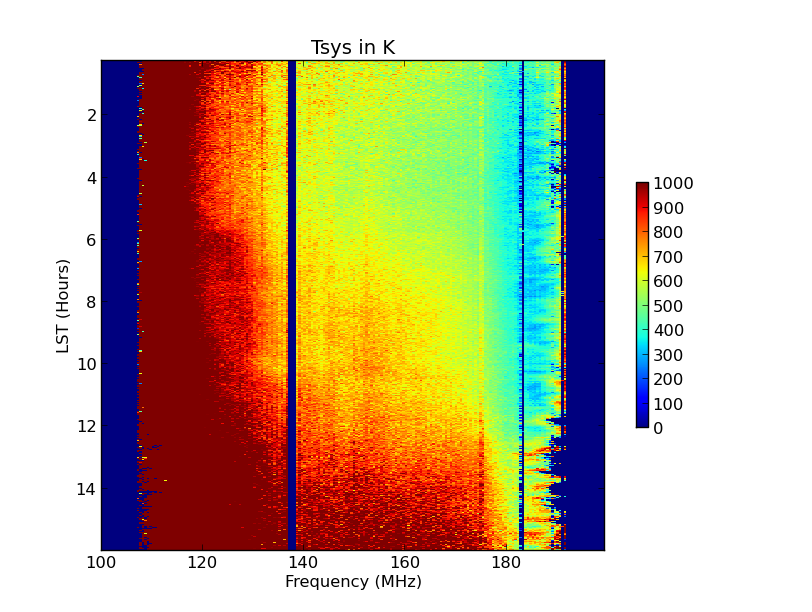
\includegraphics[width=\columnwidth]{plots/tsys_lst_freq.png}
%\caption{Tsys as a function of lst and frequency. The cold spot resides in the
%lst range of 1-7hours.}
%\ref{fig:tsys_lst_fq}
%\end{figure}

\subsection{Optimal Fringe-Rate Filter}\label{sec:frf}
%   -What is fringe rate filtering. Cite Parsons And Liu 2014.
%       --Fringe Rate filtering is nothing more then a time domain weighted
%         average per frequency of of visibilities. The filter can be applied 
%         as either a convolution in the time domain or a multiplicative fourier
%         filter in fringe rate space. 
%       --We first calculate fringe rate filter such that we upweight the more
%         sensitive fringe rates versus the not so sensitve fringe rates by
%         weighting the fringe rates for a given baseline by its beam.
%   -Effective beam areas.
%       --When fringe rate filtering, we are upweighting fringe rates that
%         are most sensitive. That is we are weighting these fringe rates by the
%         beam of a baseline. This has the effect of narrowing the effective
%         beam. It turns out that we are removing more noise than signal,
%         because we are essentially keeping the most sensitive parts of the
%         sky. This actually gives us a sensitivity boost of about a factor of
%         2. 
%   -effective integration time and number of modes. 
%       --Do calculations.
%       --Fringe rate filtering is effectively a weighted average in time and
%       thus there is an effective integration time. We can calculate this
%       integration time by noting that power (or variance) is a conserved
%       quantity. Therefore, comparing the integral of a variance=1 noise signal
%       when it is fringe rate filtered to when it is not, gives us a fractional
%       integration time. 
%           \frac{ \int_{t_{start}}^t_{end}{\sigma^{2}*F_{constant}(t)dt
%           }}{\int_{t_{start}}^t_{end}{\sigma^{2}*F_{filter}(t)dt = fraction.
%            t_int = fraction * t_start-t_end
%           Something like that.
%       --Due to the fact that fringe rate filtering is effectively averaging in
%         time, A fringe rate filter reduces the number of independent modes on
%         the sky. The number of modes in an entire day drop just 45
%         (24hrs/1900sec)  independent modes on the sky. 
%   -PLOTS: 
%       --FR filter (both in fr and time space), applied to data.
%       --Beam after fringe-rate filter. 
%       --Waterfalls.
%       -- apply filters to foreground data. Compute fr of pica and show that we
%          are not killing the sky.
%   
%   code to get the integration time of fringe rate filter. This is 1886 for channel 100
%   beam_w_fr = frf_conv.get_beam_w_fr(aa, (1,4))
%   t,firs,frbins,frspace = frf_conv.get_fringe_rate_kernels(beam_w_fr, 42.8, 401)
%   fr100 = frspace[100]
%   t_int = 42.8/n.mean(fr100)
%   

Prior to forming power spectra we need to time average visibilities that
measure the same $k$ mode on the sky. The motivation for this is that we want
to combine coherent $k$-modes on the sky before squaring to get the maximum
sensitivity. This is mathematically similar to the more traditional process of
gridding in the $uv$ plane, but for a single baseline.  However, rather
than applying a box-car average, we can apply a kernel --a so-called
'fringe-rate' filter-- that weights different temporal rates by the antenna
beam corresponding to the parts of the sky moving at the same rate.

Broadly, for a given baseline and frequency, different parts of the sky
correspond to different fringe-rates.  Maximum fringe rates are found along the
equatorial plane, where the rotation rate of the sky is highest, and zero
fringe rates are found at the poles, where the sky does not rotate and hence
sources do not move and have static fringe rates \citep{parsons_backer2009}.
However, fringe rates are not constant as a function of latitude. Bins of
constant fringe rate correspond to rings in RA and DEC, corresponding to where
the east-west projection of a baseline projected toward a patch of the sky is
constant.  We use this fact in conjunction with the average beam response for each
contour of constant fringe rate to construct our time average kernel or
``fringe-rate filter".


%[XXX this paragraph could probably go -dcj]
%As motivation, we discuss the use of fringe-rate filters in cross talk removal.
%Crosstalk is modeled as a time independent coupling of signal between two
%different signal paths. Since crosstalk does not vary as a function of time and shows up at zero fringe rate.  In this view crosstalk is a DC bias. To remove crosstalk, we can
%apply a notch filter to the fringe-rate transform of the time series visibility
%(per frequency) and inverse transform to go back into time domain. This
%interpretation of crosstalk being a DC offset jives with our method of crosstalk
%removal discussed above. In order to remove a DC offset from a time series, we
%subtract the average.
%
%Now, to optimally combine the time data we can cater our fringe-rate filter to
%upweight points of the sky that contain more signal to our instrument and down
%weight those points that do not. That is, if we weight fringe-rate
%bins by the beam, we can get a net increase in sensitivity. Roughly, all fringe
%rate bins contain the same amount of noise in them, but the amount of signal
%varies and is determined by how the primary beam illuminates the sky.
%Upweighting the bins with higher signal relative to those with less signal
%gives us a net increase in signal-to-noise, even though we are removing 
%signal by applying signal from this filter. 

Applying this filter effectively weights the data by another factor of the beam
area, changing the effective primary beam response, $A(l,m)$ .\footnote{The
angular area in equation \ref{eqn:delay_pspec} will reflect the new angular area
corresponding to the change in beam area.} \citep{parsons_et_al2015}. By
utilizing prior knowledge about the beam area we are selectively down weighting
areas on the sky contributing little signal. This results in an SNR boost of
about 2.  The net boost in SNR depends on the shape of the beam and array
declination and is functionally equivalent to the beam$^2$ weighting used in
wide-field mosaicking. It is also worth noting that, like the delay spectrum
filtering, fringe-rate filtering is implemented on a per-baseline basis.

%We implement the optimal fringe-rate filter by calculating the fringe rates at
%every point on the sky, for a given frequency, and weighting each bin by the
%beam of a given baseline. 
 We weight
the fringe-rate bins on the sky by the beam pattern at that location.
In order to obtain a smooth filter in the fringe-rate domain, we fit a
Gaussian with a hyperbolic tangent tail to this filter. We convolve the time
domain visibilities with the Fourier transform of this fringe-rate filter to
produce an averaged visibility.  The effect on the data can be seen
in Figure \ref{fig:waterfalls}.

%\begin{figure}[!t]
%\centering
%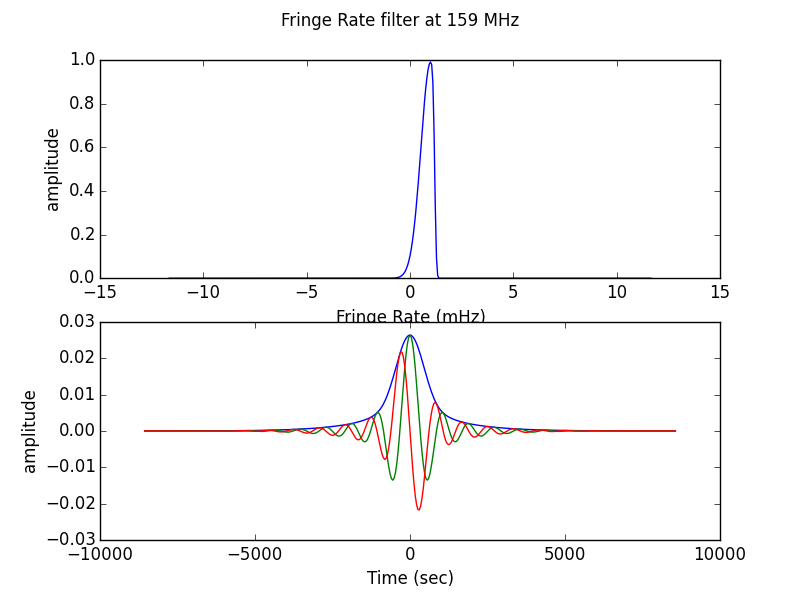
\includegraphics[width=\columnwidth]{plots/fr_filter_slice.png}
%\caption{
%slice of a fringe rate filter at a frequency of 159MHz. Top is the
%filter in fringe rate domain. The bottom consists of the corresponding time
%domain filter gotten by fourier transforming and windowing with a
%blackman-harris window to damp the tails.
%[XXX move this figure into fringe-rate filter paper]
%}
%\label{fig:fringe_rate_cut}
%\end{figure}

\begin{figure}\centering
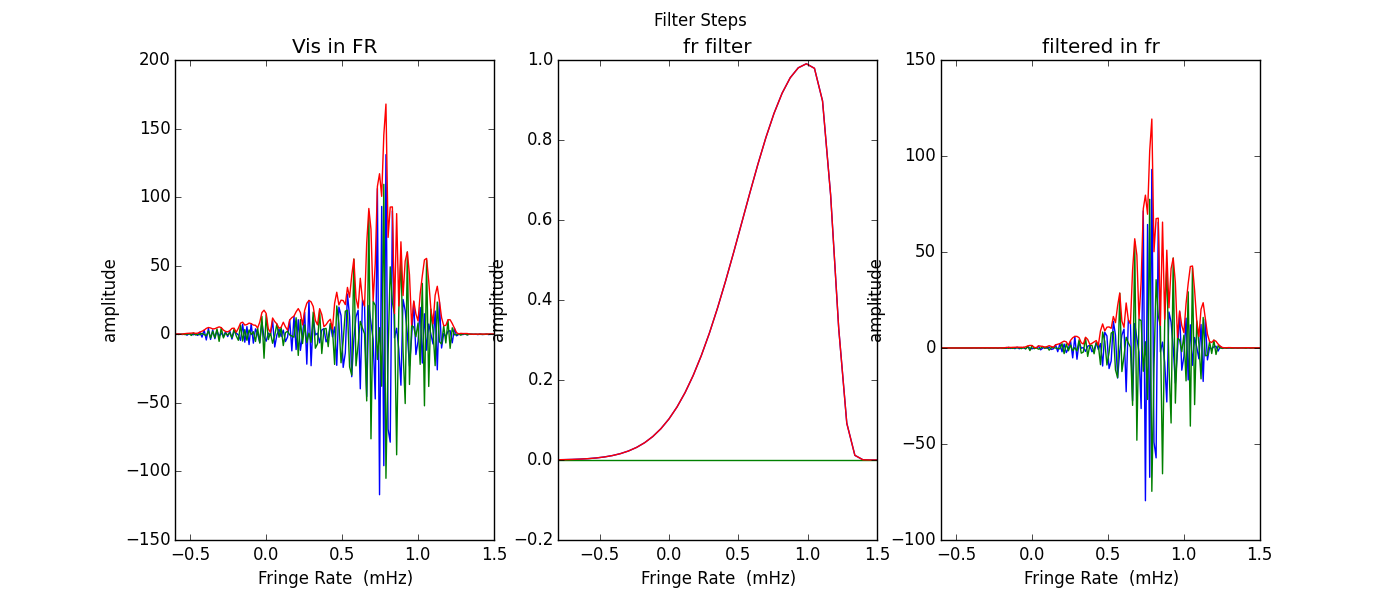
\includegraphics[width=\columnwidth]{plots/fr_preserved_signal.png}
\caption{
Fringe-rate transform of visibilities measured on the fiducial baseline at 159 MHz before (blue) and
after (red) optimal fringe-rate filtering. The fringe-rate filter (green) is normalized
to integrate to unity, but has been scaled here for legibility.
%Fringe-rate filtering at 159MHz. Fringe-rates of is defined as the rate at which
%the sky moves through the fringe pattern of a baselines fringe pattern. This is
%dependent on the frequency under consideration as well as position on the sky.
%Shown here is the fringe-rate transform (fourier transform along the time axis
%of a visibility) of unfiltered foreground contained data for a 30 m east-west
%baseline (blue). The fringe-rate filter in fringe-rate space (green) is scaled
%to highlight the shape of the filter. In practice, this filter is normalized so
%that its integral is unity.  This filter is multiplicative in this domain and
%its fourier transform convolves the time domain visibilities from which the
%unfiltered data in this plot is dervied from.  The filtered data (red) is the
%product of the unfiltered with the weights of the fringe-rate filter (green).
%Foreground signal is still retained in the final output, but signal low in the
%beam has been downweighted. For the PAPER array in South Africa, these fringe
%rates correspond to small/negative fringe rates and nearly the maximum fringe
%rates of a 30m east-west baseline. Note the maximum and minimum fringerates
%correspond to the theoretical minimum and maximum for a 30 m baseline at 159
%MHz.
}
\label{fig:fr_preserved_signal}
\end{figure}
The action of the fringe rate filter is to get an optimally weighted
sample, averaged at the longest physically possible integration time.  For the
fiducial baselines, the effective
integration time is calculated by comparing the variance statistic for a
fringe-rate filter that is a flat weighting vs that with an optimal filter
weighting as described. We apply these filters to random noise with variance 1,
without loss of generality. We can conclude that 
\begin{equation}
    t_{int} = \frac{\int{\sigma^{2}dt}}{\int{\sigma^{2}fr^{2}dt}},
\end{equation}
which evaluates to 1886 s for an optimal fringe-rate filter on the fiducial 
baseline at 150 MHz.  Over the range of frequencies used in our power spectrum
estimate, the integration times range from 1936 s to 1790 s, corresponding to an
average of 31 minutes. As a rough check, we note that this is roughly the time
it takes a source to transit through one fringe period.
Because
the fringe-rate filter integrates in time, the number of statistically
independent samples of the sky drastically decreases from 83 to $\sim2$
independent samples per hour.

%It is important to note that the fringe rate filter is removing some sky signa
%as is seen in figure \ref{fig:waterfalls}, but it is removing 
%The PAPER beam is ~60 degrees FWHM \citep{jacobs_et_al2011}, and the array is
%located at a declination of $-30^{\circ}$ the fringe rates associated with the
%low signal to noise (down in the beam) correspond to very high and very
%low/negative fringe rates.
%%Figure \ref{fig:fringe_rate_cut} shows a cut of the optimal fringe-rate filter
%%at 159 MHz for
%%a 30-m east west baseline. 
%Therefore, the implemented fringe-rate filter removes
%some sky signal, signal associated with fringe rates outside of the ranges shown
%in Figure \ref{fig:fr_preserved_signal}. Figure \ref{fig:fr_preserved_signal} shows
%that the applied filter removes sky associated with negative fringe rates and
%very high fringe rates. [XXX how does this loss compare with the delay spectrum loss?  Can't just leave this statement dangling...]
%

%\begin{figure}[h!]\centering
%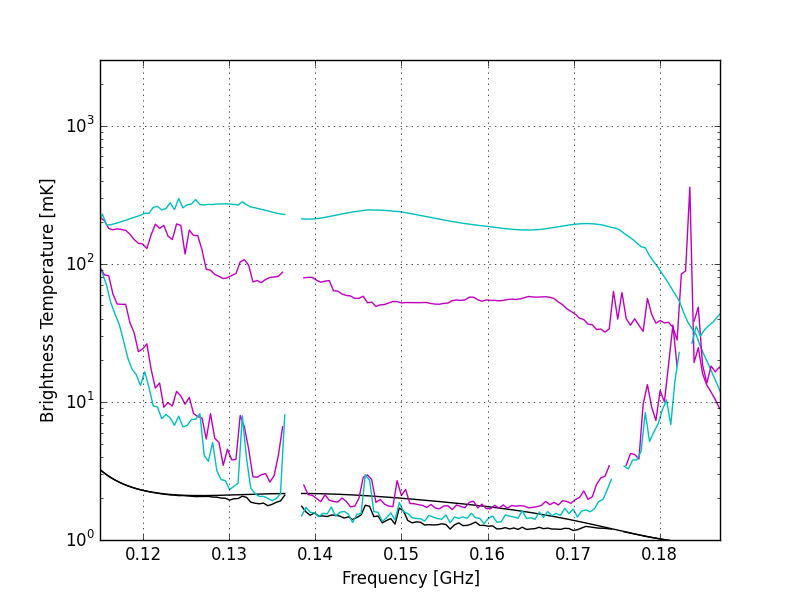
\includegraphics[width=\columnwidth, height=.8\columnwidth]{plots/noise_t_35.png}
%\caption{Estimates of noise temperature. Magenta is frequncy differenced
%estimate where the cyan is the time differenced estimate. All curves are
%averaged over all 30m east-west baselines (56) and averaged incoherently in 43s
%bins of LST from LST 3 to 5 hours with a channel bandwidth of 490 kHz.}
%\label{fig:noise_t}
%\end{figure}


%\begin{figure}[h!]\centering
%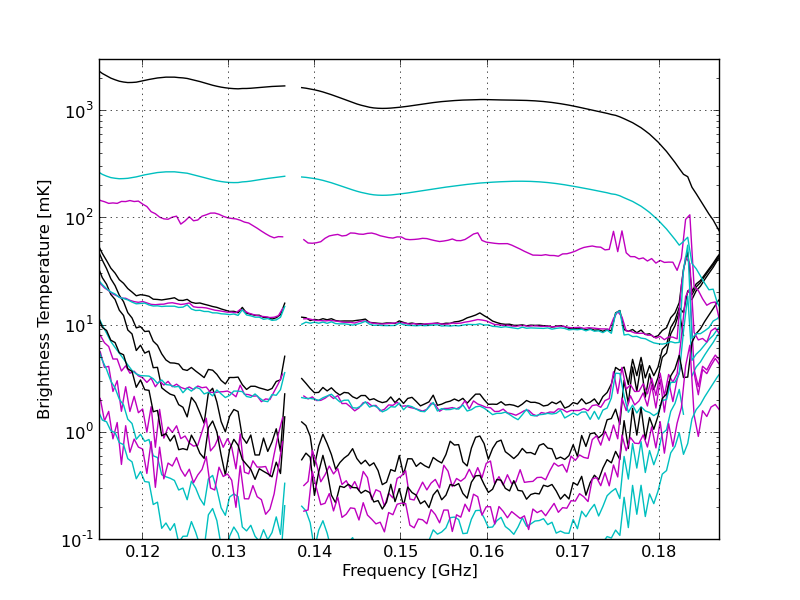
\includegraphics[width=\columnwidth, height=.8\columnwidth]{plots/noise_vs_fq_plot.png}
%\caption{Estimates of noise temperature. Magenta is frequncy differenced
%estimate where the cyan is the time differenced estimate. Averaged in LST from 3
%to 5 hours. on uv files calibrated with omnical. fg,delay filtered, baseline
%averaged, normal fringe rate filter, optimal fringe rate filtering.}
%\label{fig:noise_omni_uv}
%\end{figure}

\section{Instrumental Performance}\label{sec:instrument}
\subsection{Instrument Stability}

\begin{figure*}
\centering
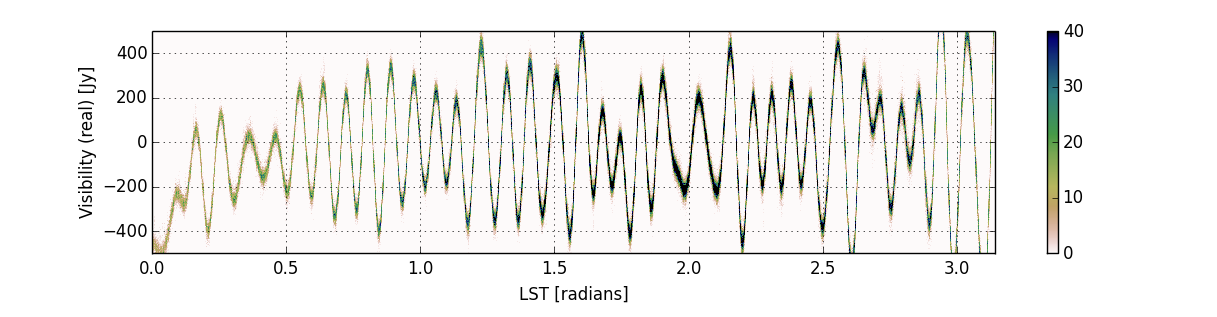
\includegraphics[width=2.3\columnwidth]{plots/density.png}
\caption{Histogram of the real component of all calibrated visibilities
measured over 135 days with every redundant instance of the fiducial baseline at 150
MHz.  Color scale indicates the number of samples falling in an
LST/flux-density bin.  This plot serves to illustrate the stability of the
PAPER instrument and the precision of calibration.
%The bulk of the samples recorded, range from an LST of 5 to
%10 hours, whilst the EoR cold spot ranges from 0 to 4 hours as seen in figure
%\ref{fig:coverage}. For the densest regions, the spread in visibility for a
%given LST sample is $\approx{100} \,\text{Jy}$. The agreement between redundant
%baselines here gives us reassurance that our baselines are actually measuring
%the same fourier modes on the sky.}
}\label{fig:density}
\end{figure*}

\begin{figure}
\centering
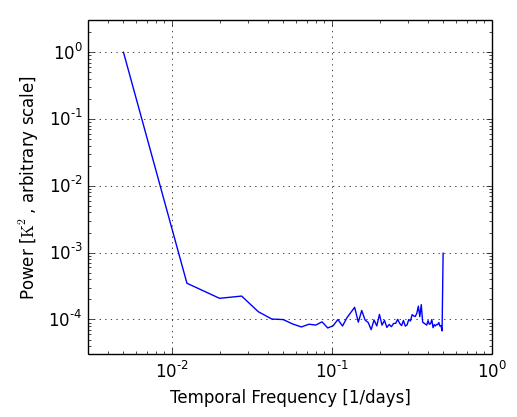
\includegraphics[width=\columnwidth]{plots/stability.png}
\caption{Power spectrum of 135 days of time-series data contributing to a single LST bin,
illustrating the stability of measurements over the observing campaign.  The excess at
2-day timescales is a beat frequency associated with the changing alignment of 
integration windows in the correlator with respect to sidereal time.  
%Demonstration of the time stability of the instrument. For a given LST
%bin, we take the day to day samples that go into that bin and determine the
%power spectrum for that time seris. Shown here is the power spectrum of the time
%series over 134 days for baseline 1\_4 at 150 MHz (XXX) averaged over 5 hours in
%LST. Power at 1/134 days$^{-1}$ is the DC bin, accumulating the average of the
%time signal. The power spectrum folows a noise like power spectrum throughout
%with a slight uptic at the temporal frequency corresponding to 2 days. This is
%due to the fact that the integration time does not fully divide out a sidereal
%day, but has a remiainder of $\frac{1}{2}$, piling up power on the everyother day
%time scale. (XXX need to be more clear here, I think. a.const.sidereal\_day/42.9
%= 2008.487, a.const.sidereal\_day/42.94 = 2006.616.)
%}
}\label{fig:stability}
\end{figure}


One PAPER design goal is the stability of the instrument between
baselines and in time. Figure \ref{fig:density} shows the visibility repeatability between 
baselines and nights as a function of LST. Specifically, we histogram the real part of
the visibilities for all redundant fiducial baselines 
in a given LST bin for foreground contained data. We see that for a
given LST bin the, spread in the value for all the baselines is $\sim$50 Jy which corresponds with our observed
$T_{sys}$ of $\sim$500K .  We get
more samples per LST bin in the range of 2--10 hours due to our observing
season, therefore the density of points in this LST region is greater, set by
the color scale. This density plot shows that redundant baselines agree very well
with one another, OMNICAL has leveled the antenna gains to within the noise.

In addition to stability between redundant baselines, we also consider the
stability in time for the PAPER instrument. In order to quantify the stability
in time we extract one channel for a given baseline for every observation day
and LST bin. We then Fourier transform along the time direction for every LST
bin and compute the power spectrum. As shown in figure \ref{fig:stability}, the
DC bin is the average of all of the days and clearly there is excess power
there. However, for time scales greater than 1 day, we see that there is little
correlation between days, showing that there are no systematics in time. The
excess on the two day timescale is caused by the changing alignment of the 42.9
second integration time scale of a visibility with that of a sidereal day. This
presents itself as a beat frequency on the two day timescale.

\subsection{System Temperature}   
During the LST binning step, the variance of the visibilities that are averaged
together for a given frequency and LST bin are recorded. Using these variances,
we calculate the system temperature as a function of LST, averaging over each
LST hour. 
\begin{equation}
    \Tsys = \frac{T_{\rm rms}}{\sqrt{\Delta\nu t}}, 
\end{equation}
where $\Delta\nu$ is the bandwidth, $t$ is the integration time, and
$T_{\rm rms}$ is the RMS temperature, or the variance statistic described above.
Figure \ref{fig:tsys} shows the results of this calculation. In this observing
season, the system temperature drops just below previous estimates of the
as in P14 and \citet{jacobs_et_al2014} at $\Tsys=500K$ at 160 MHz.
[XXX Zaki, how exactly did you get 500?  the number from P14 and J15 was 550K @ 160MHz
 This is using the variance statistic from the lst binner. The usual way to
calculate Tsys, except that there is a correction factor because we are flagging
3 sigma outside of the median. For Gaussian noise, that correction factor is
1.34 which is what I'm applying to the calculated tsys. Prior to that we were
getting a much lower tsys (350 or so). ]

\begin{figure}\centering
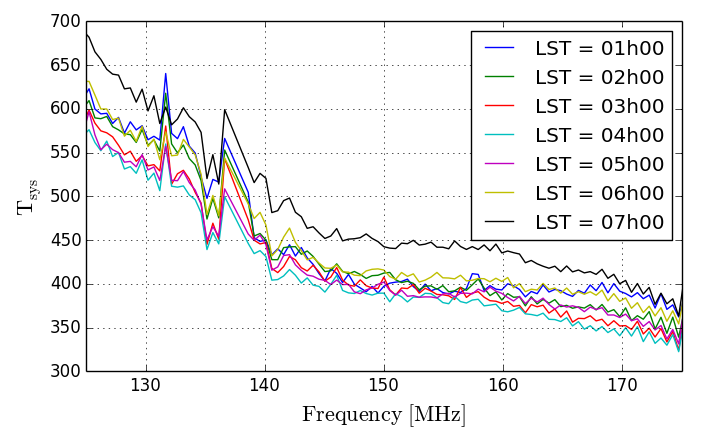
\includegraphics[width=\columnwidth]{plots/tsys.png}
\caption{System temperature, inferred from the variance of samples falling 
in an LST bin, averaged over one-hour intervals in LST.  The measured value
in the 150--160 MHz range is consistent with previous determinations of
system temperature (P14; \citealt{jacobs_et_al2014}).
%statistic calculated in every LST bin and average on hour time scales to
%estimate the $T_{sys}$ reported here. For a majority of the LST bins, especially
%those bins used in our analysis, the system temperature is about 500K at 160
%MHz, consistent with previous estimates of the system temperature.}
}\label{fig:tsys}
\end{figure}

When calculating the system temperature using the variance in the visibilities
for a given LST and frequency, we take into account the fact that we flag
3$\sigma$ outliers from the median. To calculate an effective correction factor
to account for the filtering, we assume the visibilities follow a Gaussian
distribution which would require a correction factor of 1.34 for the removal of
data points that are 3$\sigma$ above the median.

Previous estimates
of the system temperature
(P14; \citealt{jacobs_et_al2014}) relied on differencing and averaging
baselines, time samples, and/or frequency channels. The relative agreement
between these various methods of estimating the system temperature provides a
robust measure of the system temperature of the PAPER instrument. Agreement
between the instantaneous measurements of the system temperature, the LST
repetition variance, and the predicted power spectrum noise level (see below)
indicates a robustly stable system with no significant long term instability
contributing appreciable noise.



\section{Power Spectrum Analysis}\label{sec:oqe}
%   -Motivate method with discussion of empirical estimate of covariances and
%    problem of limited modes.
%       --Because we dont know the true covariances between baselines and
%         channels we have to estimate the covariances epirically from data. 
%       --We do this by taking the outer product of our data vector (consisting
%         of a visibilies for every baseline of a given unique baseline type).
%         The outer product is calculated per time sample, thus we average over
%         a "clean" (what do i mean by this?) lst range.
%       --Hence, the quality of the estimate of the covariances between
%         baselines depends on the average in time ( the ensemble average). 
%       --The fact that we do not know what the full covariance matrix looks
%         like leads to signal loss. We have an estimate of the covariance, not
%         the true covariance matrix. There is no way to truly know what the
%         covariance matrix is for our data set. 
%       --After fringerate filtering, the number of independent modes on the
%         decreases substantially because we are averaging over 1900 seconds
%         ~=31.67 minutes. Therefore the number of independent modes decreases
%         1900/(the beam in time). 
%       --In our range of lsts used, we only have roughly 20 independent
%         samples. Therefore we end up with an ill determined covariance matrix
%         to describe our data. 
%       --In addition, because of the highly redundant nature of the array,
%         the covariance matrix is highly singular and therefore not invertible.

In this section we first
review the quadratic estimator formalism, with an emphasis on our power
spectrum analysis, followed by a walk through of our application of the OQE
method to our data, and finally discuss the effects of an empirical estimate of
covariance matrices.



%
%   -Mathematics compared to ideal optimal Quadratic Estimator.
%       --In the quadratic estimator formalism, the value of the power spectrum,
%         $p_{\alpha}$  in the $\alpha^{th}$ bin is given by
%         $Mq_{\alpha}=$Mx^{\dagger}C{-1}Q_{\alpha}C^{-1}x, where x is a vector
%         containing the binned data in frequency domain, $x = V(\nu)$, C is the
%         estimate of the covariance matrix of of our data, C = <xx^{\dagger}>,
%         $Q_{\alpha}$ is defined such that $Q_{\alpha}=\frac{dC}{d\alpha}$, and
%         M is a normalization matrix that normalizes the estimator.
%       --Generally, the covaraince matrix used is the full covaraince between
%         all baselines and channels. 
%       --Because of redundancy, the matrix is singular and not invertible. We
%         therefore construct a pseudo inverse for C. In addtion to the psaudo
%         inverse we take only the auto-baseline covarainces, masking out the
%         covariances between baselines. This, is invertible. WE can thus apply
%         the inverse of C in the above equation.
%
%   -Counting of independent modes.
%       --Number of independent modes = 2*#of lst hours used in analysis. This
%         is because 1900 seconds ~ 30 minutes.
\subsection{Review of Optimal Quadratic Estimators}
We use the optimal quadratic estimator method to estimate our power spectrum as
done in \cite{dillon_et_al2013a} and \cite{liu_tegmark2011}.  Here we briefly review the
optimal quadratic estimator (OQE) formalism with an emphasis on our application
to data. The end goal of this analysis technique is to estimate the 21 cm
power spectrum, $P_{21}(\k)$, defined such that 
\begin{equation}
\label{eqn:pspec_def}
    \expval{\tilde{T}_{b}(\k)\tilde{T}^{*}_{b}(\k^{\prime})} =
            (2\pi)^{3}\delta^{D}(\k - \k^{\prime})P_{21}(\k),
\end{equation}
where $\tilde{T}_{b}(\k)$ is the fourier transform of the brightness temperature
distribution on the sky, $\expval{}$ denote the ensemble average, and
$\delta^{D}$ is the Dirac-Delta function. 


In order to make an estimate of the power spectrum, we first begin with a data
vector $\x$ which includes all of the measured  visibilities (both in time and
frequency), $V(\nu,t)$, one wishes to use in the estimate of $P_{21}$. We form
the intermediate quantity,
\begin{equation}
\label{eqn:qalpha}
    q_{\alpha} = \frac{1}{2}\x^{t}\mathbf{C}^{-1}\mathbf{Q}_{\alpha}\mathbf{C}^{-1}\x - b_{\alpha},
\end{equation}
which will be needed to form the optimal quadratic estimator of our power spectrum.
Here, $\mathbf{C}$ is the true covariance matrix of the data vector $\x$, 
$\mathbf{Q}_{\alpha}$ is the operator that takes visibilities into power spectrum
$k$-space and bins into the ${\alpha}^{th}$ bin, and $b_{\alpha}$ is the bias to
the estimate that needs to be subtracted off. This bias is the instrumental
noise bias due to the instrument itself. There is infact another source of bias
due to the foregrounds. In general, $\mathbf{Q}_{\alpha}$
is a family of matrices, one for each $\alpha^{th}$ bin (equivalent to $k$-bin
for a power spectrum analysis). It is important to note that
$\mathbf{Q}_{\alpha}$ can take on any form and be completely arbitrary. It is
the data analysts choice. However, if one is looking for the best possible
estimate of the power spectrum,  $\mathbf{Q_{\alpha}}$ generally
takes a form that is proportional to  $\mathbf{C}_{,\alpha} \equiv
\frac{\partial{\mathbf{C}}}{\partial p_{\alpha}}$, which is the derivative of
the covariance matrix with respect to the band power $p_{\alpha}$, defined
below.  Therefore, $\mathbf{Q}_{\alpha}$ encodes the response of the data
covariance matrix to the $\alpha^{th}$ bandpower. We describe our choice of this
matrix in the next section, where we describe the application of the quadratic
estimator. 

Normalizing the $\q_{\alpha}'s$ with a matrix $\mathbf{M}$, we form
the final estimate of our power spectrum,
\begin{equation}\label{eqn:pspec_norm}
    \mathbf{\hat{p}} = \mathbf{M}\mathbf{q},
\end{equation}
where $\mathbf{\hat{p}}$ is the optimal quadratic estimate of the power spectrum
for every band power $p_{\alpha}$ in $k$-space, and $\mathbf{q}$ is a vector of the
quantities in equation \ref{eqn:qalpha} for every $\alpha'th$ bin.

The bias term $b_{\alpha}$ in equation \ref{eqn:qalpha} is the instrumental
noise bias that needs to be subtracted off. However, in our analysis we are
constructing an unbiased estimator by using cross correlations between different
redundant baselines. This eliminates the need to subtract the noise bias in
equation \ref{eqn:qalpha}. However, we do not try to remove the 
foreground bias.  Due to the fact that we are using cross correlations in our
quadratic estimator of the power spectrum, equation \ref{eqn:qalpha} becomes, 
\begin{equation}\label{eqn:qalpha_unbiased}
    q_{\alpha} =
\frac{1}{2}\x_{1}^{t}\mathbf{C}^{-1}\mathbf{Q}_{\alpha}\mathbf{C}^{-1}\x_{2} - b_{\alpha},
\end{equation}
where $x_{1}$ and $x_{2}$ are visibility vectors that correspond to two
different redundant baselines. This cross correlation is the key to obtaining a
zero bias estimate of the power spectrum. 

The normalization matrix above is defined such that
\begin{equation}\label{eqn:window_def}
    \mathbf{W} = \mathbf{M}\mathbf{F}, 
\end{equation}
where $\mathbf{F}$ is the Fisher information matrix, given by
$\mathbf{F}_{\alpha\beta} =
\frac{1}{2}tr(\mathbf{C}^{-1}\mathbf{Q}_{\alpha}\mathbf{C}^{-1}\mathbf{Q}_{\beta})$
and $\mathbf{W}$ is the window function matrix. The window functions measure the
degree to which power from $k$ bins couple into the measurement of the power
measured in the $\alpha$'th $k$ bin. Specifically, 
\begin{equation}\label{eqn:true_pspec_2_est_pspec}
    \hat{\mathbf{p}} = \mathbf{W}\mathbf{p}, 
\end{equation}
where $\mathbf{p}$ and $\hat{\mathbf{p}}$ are vectors of the true power spectrum and our
estimate of the power spectrum for every $\alpha$'th bin, respectively. Note
that the window functions are normalized such that the rows of $\mathbf{W}$ sum
to unity.

%   -Cholesky Decomposition and window functions.
%       --The optimal window functions (that minimize the vertical error bars of
%       the estimate, are given by the inverse of the Fisher matrix. However,
%       there is a trade off such that this incorporates information from all of
%       the k-modes. 
%       --Some other choices of the window functions are the square root of the
%       fisher matrix or the identity. 
%       --We use the cholesky decomposition of the Fisher Matrix such that we
%       can write F = LL^{\dagger}, where L is a lower triangular matrix. This
%       is possible for any hermitian positive-definite matrix.
%       --We use L for our window functions because for every k-bin, it does not
%       use information from the k-bins below it. And thus there is no mixing of
%       modes lower than it. 
%       --This is particularly important because it doesn't insures that there
%       is no leakage of the modes within the horizon to modes outside of it.         
%
The normalization matrix is the analysts choice, and is the last chance to
weight the measurements in the estimates of the power spectrum; it is
essentially a re-binning of the data. One choice that can be made is to pick
$\mathbf{M} = \mathbf{F}^{-1}$ implying that $\mathbf{W} = \mathbf{I}$. This
window function is a delta function window such that every band power does not
contain leakage from other band powers, and therefore the estimates are well
localized and contain power from only that bin. However, this has the down side
that the error bars are large.  On the other hand, choosing the identity
normalization such that the window functions are given by the Fisher matrix,
leads to the smallest possible error bars, with the consequence that every
band power is coupled to every other band power.  
[XXX this bit needs work.. what was I trying to say with this?]
The choice of $\mathbf{M} =
\mathbf{D}$, where $\mathbf{D}$ is a diagonal matrix, produces the smallest
possible error bars [XXX cite result]. $\mathbf{D}$ is diagonal and not the
identity because the window functions are normalized such that the rows of the
matrix sum to unity.  

In addition to calculating the window functions, we can also calculate the error
correlations that correspond to a given window function. In order to see the
effect of the normalization matrix on the error correlations we start by looking
at the covariance of the band power estimates, namely, 
\begin{equation}\label{eqn:err_cov}
    \boldsymbol \Sigma = \text{Cov}(\hat{\mathbf{p}}) = \expval{\hat{\mathbf{p}}\hat{\mathbf{p}^{\dagger}}} -
             \expval{\hat{\mathbf{p}}}\expval{\hat{\mathbf{p}}}^{\dagger}.
\end{equation}
Since $\phat = \mathbf{M}\qhat$, it is easily shown that 
\begin{equation}
    \Sigma = \mathbf{M}\mathbf{F}\mathbf{M}^{\dagger},
\end{equation}
where $\mathbf{F}$ is the Fisher matrix. The error correlation matrix describes
how correlated the errors between modes are in the final power spectrum result.


\subsection{Application of Optimal Quadratic Estimators}
\label{sec:oqe_app}
% A walk through of the application to the data.

Here we describe the specifics of our application of the optimal quadratic
estimator formalism to measure the power spectrum. The form of our estimator is
based on the delay spectrum technique described in P12a. The estimate of the
power spectrum using this approach can be written as 
\begin{equation}\label{eqn:delay_pspec}
    \hat{P}(\mathbf{k}_{t\tau}) =
\Big(\frac{\lambda^{2}}{2k_{B}}\Big)^{2}\frac{X^{2}Y}{\Omega
B}\expval{\tilde{V}_{i}(t,\tau)\tilde{V}_{j}^{*}(t,\tau)},
\end{equation}
where $V_{i}(t,\tau)$'s are the delay spectra of baseline visibilities, $X$ and
$Y$ are the constants that convert from angles and frequency to the co-moving
coordinate, respectively, $\Omega$ is the power squared beam (see Appendix B of
P14), and $B$ is the bandwidth. The expectation value represents the ensemble
average over instantaneously redundant baselines, and hence over a single
Fourier mode. One of the important assumptions in the estimation of the power
spectrum in this was is that delay modes are a very good approximation to
line-of-sight Fourier modes, which holds for the fiducial baselines used in this
analysis (P12b). Due to the chromaticity of an interferometer, this is in
general not valid assumption and depends on the length of the baseline.

First, we describe our data set used in the application. Our data set consists
of visibilities as a function of frequency and time for each baseline in the
array. In estimating the power spectrum we use specific redundant groups baselines,
applying the analysis to different groups separately. In the
description what follows we use the fiducial baselines,
but we apply the same analysis to each of the redundant groups described in Section \ref{sec:observations}.
Measurements obtained with the different redundant groups are combined in the averaging and
bootstrapping over modes in the estimate of the final power spectrum.  Focusing on the fiducial
baselines, our data vector becomes a list of visibilities
such that
\begin{equation}
\label{eqn:xvectdef}
\mathbf{x} = \left( \begin{array}{c}
V (t_{1}) \\
V (t_{2}) \\
\vdots \\
\end{array}
\right), 
\end{equation}
where, $V(t_{i})$ is the visibility of a baseline, indexed by LST bin,
belonging to the redundant baselines under consideration. Each visibility
contains 10 MHz of bandwidth centered at 151.5 MHz, amounting to 20 channels. 
Notice that we have only included data from one baseline, which is looking ahead
to the application of the method our data. We in effect apply the quadratic
estimator on a per baseline basis and sum the baselines together to get our
final estimate. The important point is that the data vector is in frequency
space, where our final power spectrum estimate is in Fourier space. 

This leads to the description of the matrix that takes the data vector,
$\mathbf{x}$, and transforms it into something that is in the power spectrum
domain, $\mathbf{Q}_{\alpha}$. Because our data matrix is in frequency domain,
we need a way of transforming that data into $k$-space, and specifically into
the line of sight $k_{\parallel}$-modes. As shown in P12b,
line of sight $k$-modes are approximated by delay modes for short baselines and
therefore the $\mathbf{Q}_{\alpha}$ should encode the delay transform. This is,
in fact, the form of this matrix we use; we encode the delay transform in to
the $\mathbf{Q}_{\alpha}$ by taking the outer product of a sine wave with a
given delay mode, $\alpha$,  with itself.  Therefore, we construct a family of
$\mathbf{Q}$ matrices, each with a specific delay transform measuring a single
delay mode. 
%[ include plots of application of Q to data?] ARP: don't think so: too many plots

According to equation \ref{eqn:qalpha}, there is one more fundamental piece of
information we require, the covariance matrix, $\mathbf{C}$. The covariance
matrix of the data vector $\x$, by definition, is the ensemble average of
$\x\x^{t}$, namely $\mathbf{C} = \expval{\x\x^{t}}$. However, due to our limited
universe, we empirically estimate the covariance matrix by taking the time average of the
quantity $\x\x^{t}$ over a range of LSTs. We discuss the implications of
empirically estimating the covariance matrix in a later section, due to the fact
that the cusp of the problems with signal loss are attributed to this estimate.

The covariance matrix plays an important role in the optimal quadratic estimate
of power spectra. For ease of notation, let us define 
\begin{equation}\label{eqn:z}
    \mathbf{z} =  \mathbf{C}^{-1}\mathbf{x},
\end{equation}
which is the weighting of the data by the inverse covariance. This is a crucial
step in the analysis since it suppresses covariant signal between $k$-modes by
down weighting that signal. The application of the covariance matrix to data has
the same general suppression, however, different data sets have different
covariances. Figure  \ref{fig:inv_cov} shows what happens when one applies the
inverse covariance to a data vector that contains foregrounds, and therefore
highly covariant,  and one which has the foregrounds removed via that wideband
delay filter described in Section \ref{sec:wbd_filtering}.  In the figure, the
top row corresponds to the data vector $\mathbf{x}$, which is a waterfall of
the visibilities with frequency on the $x$-axis and time on the $y$-axis. The
middle section shows the empirical estimate of the covariance by taking the
outer product of $\x$ with itself and collapsing over the time axis. Finally,
the last row is the application of inverse covariance weighting to the data,
namely $\mathbf{z}$.

Applying the inverse covariance to $\x$ down weights the
strongest eigenmodes of the covariance matrix, $\mathbf{C}$, and up-weights the
weakest eigenmodes. In comparison, for random white noise, the optimal
weighting scheme is inverse variance weighting, which leads to the smallest
error bars. For an infinite sample of random white noise, the covariance matrix
would be diagonal and applying the inverse covariance would be identical to
inverse variance weighting. The diagonal of this inverse covariance matrix are
the eigenvalues and correspond to the eigenmodes. Therefore, the most
down-weighted modes correspond to the largest eigenvalues of $\C$, and hence the
strongest modes.  Similarity, applying the inverse covariance to the baseline
data vector, $\x$, the strongest modes get down weighted. 

Looking at $\mathbf{z}$ in figure \ref{fig:inv_cov} for the visibilities that
still contain foreground signal (left half) shows the down weighting of
the strongest modes which correspond to foregrounds. The strongest modes here,
are the strongest eigenmodes of the covariance matrix. Figure
\ref{fig:eigs} shows the eigenspectrum and the four strongest eigenmodes of a
covariance matrix derived from a data vector with foregrounds. As seen four
strongest eigenmodes are highly suggestive of smooth spectrum sources. In
contrast, the right half of figure \ref{fig:inv_cov} shows the application of
inverse covariance weighting to data which has the wideband delay filter applied
to remove smooth spectrum foregrounds. Applying the covariance, is up-weighting
the weakest modes in the data and since the strongest, foreground, modes have
been removed we are seeing the up-weighting of the noise. This is paralleled by
looking at the eigenspectrum and strongest eigenmodes of the foreground-less
covariance matrix in which the strongest modes do not have any coherent
structure to them and can be considered noise-like.


\begin{figure*}\centering
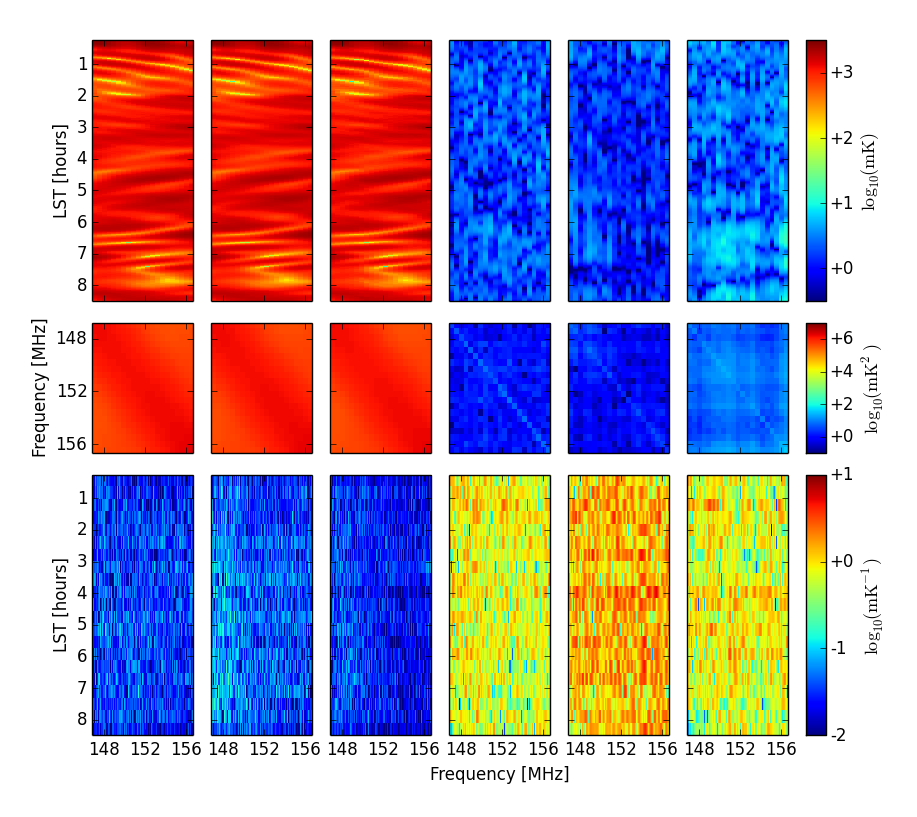
\includegraphics[width=2\columnwidth]{plots/inv_cov.png}
\caption{
Visibilities before (top row) and after (bottom row) inverse covariance weighting.
Signal covariance (middle row) is estimated empirically, averaging over LST.
The three left/right columns show visibilities from
instantaneously redundant baselines before/after delay filtering, respectively.
} \label{fig:inv_cov}
\end{figure*}

\begin{figure*}\centering
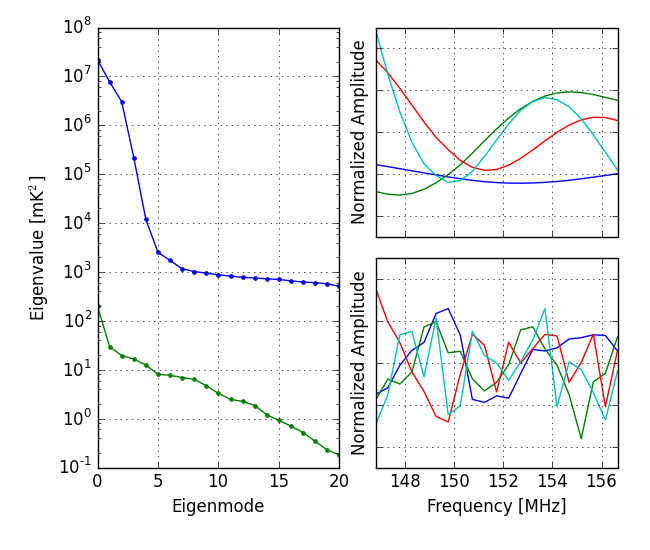
\includegraphics[width=1.5\columnwidth]{plots/eig.png}
\caption{
Eigenspectrum of covariance matrices (left) empirically estimated 
from visibilities before (blue) and after (green) delay filtering.
The four strongest eigenmodes of the filtered/unfiltered data are plotted
on the top/bottom panels on the right, respectively.
%The eigenspectrum for the foreground contained data
%has a sharp decline for the first few eigen modes and levels of at around 1 K,
%suggesting that most of the variation in the data are only described by a
%handfull of eigenmodes. The four strongest corresponding eigenmodes (top right
%panel) shows that these modes are smooth spectrum modes, suggestive of smooth
%foregrounds.  Contrastingly, the eigenspectrum for delay filtered data, in which
%foregrounds are heavily filtered, steadily decreases suggesting that there are
%not a few modes that mostly describe all of the variation in the data. This is
%paralleled in the strongest eigenmodes for this filtered data (bottom right
%panel) and there is no coherent structure to any of these modes. 
} \label{fig:eigs}
\end{figure*}

As noted in the previous section, we use cross correlations between baselines
and times to construct an unbiased estimator of the power spectrum. This results
in applying equation \ref{eqn:qalpha_unbiased}, without the bias term, namely, 
\begin{equation}
\label{eqn:qalpha_nobias}
    q_{\alpha} =
        \frac{1}{2}\x_{1}^{t}\mathbf{C}^{-1}\mathbf{Q}_{\alpha}\mathbf{C}^{-1}\x_{2}.
\end{equation}
Here, $\x_{1}$ and $\x_{2}$ are data vectors which have uncorrelated noise
properties leading to the removal of the bias term. As mentioned in section
\ref{sec:wbd_filtering}, we have constructed two LST binned data sets, which are identical
in sky signal, but have varying noise properties, owning to being created with
every other day of observation.  This allows us to construct unbiased (in
instrumental noise) quadratic estimator of the power spectrum, but will allow
for a foreground bias if residual foregrounds are still in the data at some
significant level after the application of the delay filter.


Firstly, we divide the baselines into five different groups without repeating
baselines. For each bootstrap, as discussed below, we randomly sample with
replacement baselines from each group. When computing the estimate of the power
spectrum, we only cross multiply the baselines between groups and never compute
the auto power, minimizing the bias.

Secondly, we use the data from the two LST binned data sets which were created
by binning every other days into the same LST grid. We refer to these data sets
as the ``even" and ``odd" data sets. When constructing our estimate of the power
spectrum, we use baselines from these two data sets on either side of the
$\mathbf{Q}$ matrix, being careful not to include the same baseline from the
same data set on both sides. This is another axis on which we are trying the
remove the noise bias.


Taking the above two caveats in to consideration, we then construct our optimal
estimator by applying equation \ref{eqn:qalpha_nobias} to the baseline data. In
order to obtain the final estimate of the power spectrum, we average all of the
baselines together as a function of time, measuring one power spectrum per LST
bin. Therefore, because we are using only the auto covariances to weight the
data vector, that is we are not taking into account the baseline-baseline
covariances when weighting the data, only the frequency-frequency covariances
between channels. This is a major difference between the analysis described in
P14, where baseline-baseline covariances were being taken into account. To
understand the application of this quadratic estimator formalism to the data,
let us begin by defining 
\begin{equation}\label{eqn:presum_oqe}
    \mathbf{z}^{r}_{A} = \sum_{i\in{A}} \mathbf{C}_{i}^{-1}\mathbf{x}_{i},
\end{equation}
where $r$ denotes either \emph{even} or \emph{odd} depending on the LST data set
used and $A$ denotes the group of baselines under consideration. Notice that the
sum occurs over the baselines within a group for a given LST dataset. Using this
definition, our final estimate of the intermediate quantity, $\mathbf{q}$, is
given by 
\begin{equation}\label{eqn:presum_qalpha}
    \qhat_{\alpha} = \sum_{\substack{A,B,r,s\\r\ne{s},A\ne{B}}}\mathbf{z}^{r\dagger}_{A}\mathbf{Q}_{\alpha}\mathbf{z}^{s}_{B},
\end{equation}
where the sum occurs over $A,B,r,s$ where $r\ne{s}$ and $A\ne{B}$. Furthermore,
since our $\mathbf{Q}_{\alpha}$ simply encodes a delay transform, it becomes
separable such that, $\Q_{\alpha} =
\mathbf{m}_{\alpha}^{\dagger}\mathbf{m}_{\alpha}$, where $\mathbf{m}_{\alpha}$ a
complex sine wave of a specific frequency corresponding to delay mode $\alpha$.
This is a consequence of approximating delay modes as Fourier line of sight
modes, which is a valid approximation for the short baselines under
consideration. If this were not the case, $\Q$, would not be as simple as this
and would be required to take in to account the coupling between delay modes. 
Under this approximation, equation \ref{eqn:presum_qalpha} becomes
\begin{equation}
    \qhat_{\alpha} =
\sum_{\substack{A,B,r,s\\r\ne{s},A\ne{B}}}\mathbf{z}^{r\dagger}_{A}\mathbf{m}_{\alpha}^{\dagger}\mathbf{m}_{\alpha}\mathbf{z}^{r}_{A}.
\end{equation}

After forming intermediate quantities, we must normalize our power spectrum
estimate to obtain sensible estimates on the power spectrum. As noted above, the
normalization occurs by the $\mathbf{M}$ matrix in equation
\ref{eqn:pspec_norm}, and can be any matrix of our desire. 
Even though the choices of the normalization matrices described above have some
good properties, e.g. small error bars and no leakage, we opt for a different
choice of window function as follows. We first take the Cholesky decomposition of
the Fisher matrix such that $\mathbf{F} = \mathbf{L}\mathbf{L}^{\dagger}$, where
$\mathbf{L}$ is a lower triangular matrix\footnote{This is possible for any
positive definite matrix}. Then, we choose ${\mathbf{M}} = \mathbf{L}^{-1}$ to
be our normalization matrix. In this case, the window function matrix becomes,
$\mathbf{W}=\mathbf{L}^{\dagger}$. Note that we first reorder the rows of the
Fisher matrix before decomposing into a product of upper and lower triangular
matrices. The reordering scheme puts higher $k$-modes first and lower ones last
in the list. After decomposing, this choice of $\mathbf{M}$ matrix has the
effect of only coupling modes exterior the $\alpha$'th mode only to the band
power in $\alpha$  for the final estimate of the power spectrum.  With the
ordering described above, this has the consequence of not coupling the modes
inside the horizon in to measurements of band powers outside the horizon. Figure
\ref{fig:window_func} shows these window functions. 

\begin{figure}\centering
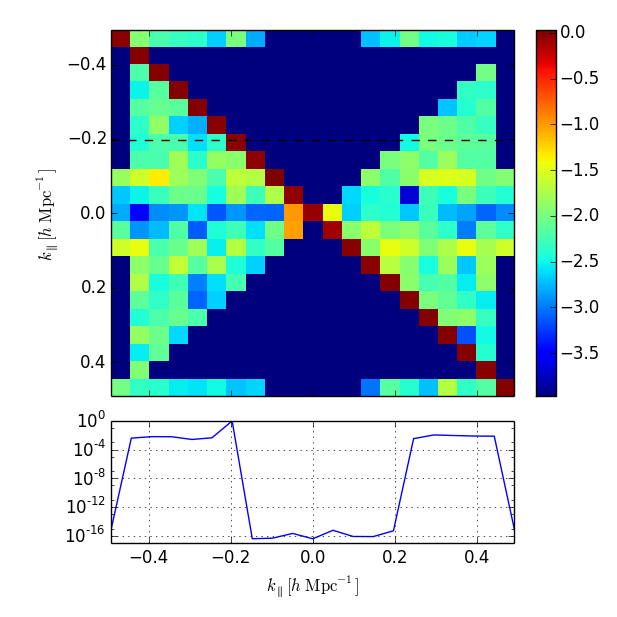
\includegraphics[width=\columnwidth]{plots/window.png}
\caption{
The window function matrix $\mathbf{W}$, as defined in equation \ref{eqn:true_pspec_2_est_pspec}.
The $i^{\rm th}$ row corresponds to the window function
used in the estimate of the power spectrum for the $i^{\rm th}$ $k$-mode.
Color scale indicates $\log_{10}\mathbf{W}$.
The inset plot illustrates the window function along the dashed line in the upper panel.
As described in Section \ref{sec:oqe_app}, $\mathbf{M}$ in equation \ref{eqn:window_def} has been chosen so that
each window function peaks at the waveband while achieving a high degree of isolation from
at lower $k$-modes that are likely to be biased by foregrounds.
}\label{fig:window_func}
\end{figure}



In addition to the nice properties in the estimates of the power spectrum given
by the above normalization and window function matrix, there is another nice
property about the choice of normalization which corresponds to the error
correlation. Using the choice of normalization matrix described above, we have
that \begin{equation} 
    \Sigma = \mathbf{L}^{-1}\mathbf{L}\mathbf{L}^{\dagger}\mathbf{L}^{-\dagger}
           = \mathbf{I}.
\end{equation}
Therefore, for $\mathbf{M}=\mathbf{L}^{-1}$, the error correlations are
proportional to the identity matrix. Proportional to the identity matrix because
our choice of $\mathbf{M} \propto \mathbf{L}^{-1}$ due to the normalization
criteria. Each row of $\mathbf{M}$ are normalized to sum to 1 and therefore,
the error correlation, or covariance of the estimate of our band powers, is only
proportional to the identity matrix, and hence diagonal. This is a very well
behaved property that implies that the error bars between band powers are not
correlated and hence the error bar on every measurement is independent from on
one another. [XXX contrast to the blackmann-harris window function in which
band powers nd errors were correlated with one another. maybe?].

The Fisher matrix is a key component in the above analysis and contains a
wealth of information about the amount of information in each $k$-mode. The
Fisher matrix is shown in figure \ref{fig:fisher}, represents the amount of
information there is in every $k_{\parallel}$ mode. The Fisher matrix is derived
using all of the baselines, not just a baseline pair and consists of all of the
information contained in the estimate.

\begin{figure}\centering
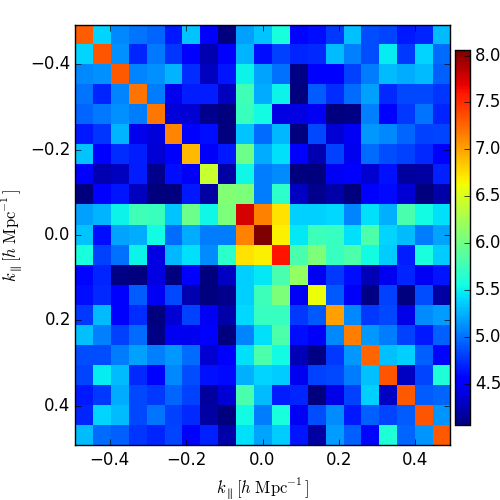
\includegraphics[width=\columnwidth]{plots/fisher.png}
\caption{
Fisher information matrix, $\mathbf{F}=\langle\qhat\qhat^\dagger\rangle$, for the quadratic estimator described in
equation \ref{eqn:presum_qalpha}, applied to delay-filtered data. 
Color scale indicates $\log_{10}\mathbf{F}$.
$\mathbf{F}$ is artificially high for the center three $k$-modes whose amplitudes have been heavily
suppressed by the delay filter.
}

%XXX This part needs work. My understanding of the Fisher Matrix is still
%undeveloped. Noisier modes are upweighted in k-space? 

%Fisher matrix captures the covariance of the intermediate $\qhat$'s with one
%another. The diagonal of the Fisher matrix, gives the auto-covariance of the
%$\qhat$ with itself. The first mode in the horizon has a bulk of the signal
%removed via the dleay filter and since the Fisher matrix takes into account
%inverse covariance weigthing of the data, it upweights those modes.
%Contrastingly, the second mode in the horizon and the first mode outside the
%horizon is suppressed because of some possibly residual signal left by the delay
%filter and kicking up of signal to outside of the horizon. The excess covariance
%cross in the Fisher matrix comes from the inverse covariance weighting applied
%to the data in the calculation of $\qhat$, which downweights the signal.}
\label{fig:fisher}
\end{figure}


\begin{figure*}\centering
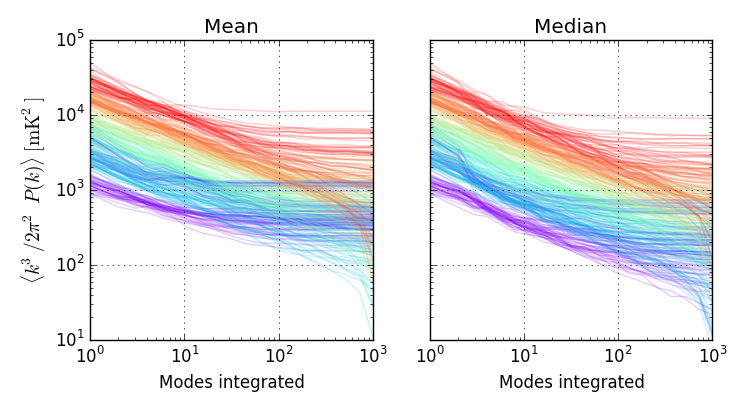
\includegraphics[width=1.8\columnwidth]{plots/pspec_variance.png}
\caption{
Cumulative mean (left) and median (right), as a function of number of modes,
of power spectrum band power for
$k_\parallel$ modes ranging from $-0.49$ (red) to $0.44\hMpci$ (violet).
This Allen variance plot shows modes averaging down as the square root of
number of modes combined until a signal floor is reached.  The difference in
behavior between the mean and median for several modes indicates non-Gaussianity
in the distribution of values, likely as a result of foreground contamination.
%Plotted is the cumulative mean for band powers at a given $k$-mode,
%where the colors indicate the mode being integrated, with blue being the most
%interior modes and walking out to the exterior modes in green; red being the
%modes in the middle. On the right is the same plot, except using a median
%instead of the mean as the statistic. The behaviour of either of these
%statistics is very similar with modes that bottom out on something and there
%modes that seem to take a dive as more modes are used. Assuming Gaussian
%statistics, there is an overall correction factor of 1.4 for using the median
%statistic relative to the mean.}
}\label{fig:pspec_variance}
\end{figure*}


\subsection{Covariance Matrix and Signal Loss}
\label{sec:sigloss}
%Covariance matrix nuances.
%   -describe covariance matrix and data vectors.
%   -How we get the covariance matrix. 
%   -eigenvalue decomposition.
%mode counting and nonsingular-ness.
%   -Count independent modes.
%   -covaraiance is independent only if we have enough indendent modes.
%   -inverse covariance is tricky because of this. 
%   -happy coincidence?
%

We now discuss the issues of empirically estimating the covariance matrix from
the data. The covariance matrix is defined as the ensemble average of the outer
product of vector with itself. In our case, 
\begin{equation}
    \C = \expval{\x\x^{\dagger}}, 
\end{equation}
where $\x$ is the data vector used in the analysis. Specifically, this data
vector consists of visibilities for a single baseline type, with 20 frequency
channels spanning 10 MHz of bandwidth
centered at 151.72 MHz, for all integrations.
Since we do not have a priori knowledge of the covariance matrix, 
we instead estimate it empirically from the data, averaging over the time
axis to derive the estimated covariances among the 20 frequency channels. In our
analysis the time average runs from 0 to 8:30 LST hours. Our analysis method
for calculating the power spectrum requires the inverse of the covariance
matrix to weight the data. Therefore, the empirically derived covariance matrix
here, must be invertible, which occurs only if $\C$ is a rank-N matrix, where N
is the number of rows or columns. In our particular case, N=20.

There are a few fundamental problems that occur when estimating the covariance
matrix in this way. As noted in section \ref{sec:frf} the optimal fringe-rate
filter corresponds to averaging time samples for 31 minutes. Over the LST range
used in this analysis, this corresponds to on the order of 20 statistically
independent modes in our data after fringe-rate filtering. This is a fundamental
limit of the amount of information we have in our measurements. Coincidentally,
the covariance matrix for a given baseline is an $N_{ch} \times N_{ch}$ matrix,
where $N_{ch}=20$.  Therefore, the covariance matrices for every baseline are,
in fact, invertible in most cases,  because they are full rank and contain 20
statistically independent measurements of the sky. The covariance matrix is thus
invertible and can be used to inverse covariance weight the data.

The optimal quadratic estimator has an application of the inverse covariance
matrix to data vector $\x$. Applying an inverse covariance matrix to the data it
is derived from has the effect of weighting the data by the covariance matrix.
Therefore strong modes, corresponding to the eigenvectors of the covariance
matrix, are down-weighted in this scheme as seen in figure \ref{fig:inv_cov}.
For foreground contained data, the strong modes correspond to the smooth
spectrum foregrounds, and therefore the covariance matrix is highly covariance
since all of the frequency channels are correlated with one another. However,
for foreground filtered data, the strongest modes correspond to modes that
resemble residual foreground in the data. It is important to note that inverse
covariance weighting is a powerful tool as seen by looking at the three
baselines used in figure \ref{fig:inv_cov}. For the baseline data vector with
the least amount of noise in the delay filtered plot (right half, middle
column), we can see that weighing by the inverse covariance up-weights modes in
this baseline as compared to the other baselines, which have a slightly higher
noise in the original data vector. This is even paralleled in the foreground
contained data.
%
%   -Potential for signal loss.
%       --In a traditional OQE method, the process is lossless by construction.
%         Because we are tweaking this method, and the fact that we have non
%         Gaussian systematics in our data, there is a potential for signal
%         loss. 


Another problem that occurs from empirically estimating covariances is that it
leads to models of the covariance matrix that over-fit the noise. Hence, when used in conjunction with the
data, it doesn't perfectly remove covariances between channels and baselines and
has the ability to remove signal from the data. [XXX Need to be more clear on
this point ]


%   -Simulations
%       --In order to show the degree that there could be signal loss, we run
%         simulations to show that an EOR -like signal does pop come out in our
%         data. 
%       --We inject a common eor like signal, a complex random white noise
%         signal, on to all of the baseline data used in this analysisi for a
%         given time. This signal is fringe rate filtered to match the data and
%         therefore, the number of independent modes matches the input data. 
%       --We run this simulation for varying signal levels, showing that this
%         signal can infact be recovered, with some signal loss.
%       --These simulations show that there is signal loss in this method.
%         However, if the signal was bright enough, we would be able to see it.
%         Since we don't see signal in the actual data, we can say that we have
%         not detected the EOR signal yet.

In theory, optimal quadratic estimators for the power spectrum described above are a
lossless operation. However, this is only true if we have all the information
needed to apply this method. As discussed [XXX where?], one of the major unknowns we have in our
estimate is the covariance matrix that describes the covariances in the data
due to the instrument and sky signal. Not knowing the true
covariances leads to signal loss in the final estimate of the power spectrum.
Here, we describe estimate the signal loss associated with the empirical
estimates of the covariance matrix.

In order to characterize
the signal loss, we simulate visibilities for spatially Gaussian signal with a
flat amplitude in $P(k)$ that rotates with the sky, and is fringe-rate filtered in
the same way as the data.  This signal is injected on top of the data,
measuring the output signal power spectrum and comparing it to the input signal
power spectrum for various signal amplitudes.  We perform this injection
for 40 draws at each signal level.
Figure \ref{fig:signal_loss} shows the resultant signal loss associated
with estimating the covariance matrix from the data.  Error bars were
obtained through bootstrapping.  
[XXX need more discussion of what the plot means]

\begin{table}[htdp]
\caption{SIGNAL LOSS VERSUS ANALYSIS STAGE}
\begin{center}
\begin{tabular}{rll}
Analysis Stage & Typical Loss & Maximum Loss \\
\hline
Bandpass Calibration &  $< 2 \times 10^{-9}$ & 0.03 \\
Delay Filtering & $1.5\times10^{-5}$ & 0.048 \\
Quadratic Estimator & $<0.02$ & 0.89 \\
Median of Modes & 1.4 & 1.4 \\
\end{tabular}
\end{center}
\label{tbl:sigloss}
\end{table}%

%XXX Need to claim that we ran an end to end test.

%XXX Carina's Text of the eor model goes here.
%The model eor signal used was a simulation of a flat power spectrum, in P($k$),
%from $k$-modes ranging from .1-10 $\text{hMpc}^{-1}$. From this an angular power
%spectrum is computed (\cite{datta_et_al2007, lewis_challinor_2007}), ensuring
%correlation in frequency/redshift for the power spectrum maps. Visibilities are
%then simulated for this power spectrum map by explicitly integrating fringes on
%the sky every 42.8 seconds for an East-West baselin of 30 m.

%In order to effectively characterize signal loss in our analysis pipeline, we
%simulate visibilities that accurately capture the instrumental effects of PAPER
%for the frequency bins used in the analysis. The signal injected into the
%simulation is comprised of two components - an artificial power spectrum P(k)
%and frequency extrapolated galactic foregrounds from the Global Sky Model (GSM)
%(de Oliveira-Costa et al. 2008). The injected power spectrum is flat in P(k) for
%a k-range of 0.1-10 $\text{hMpc}^{-1}$, and the angular power spectrum is computed from
%this (\cite{datta_et_al2007, lewis_challinor_2007}), ensuring correlation in
%frequency/redshift for the power spectrum maps. PAPER visibilities are simulated
%for both the GSM and power spectrum maps by explicitly integrating fringes on
%the sky every 42.8s for an East-West baseline of 30m.


%Need to argue that the detections are not Gaussian and therefore are not eor
%detections.


%   -Maybe : Problem of low noise measurements in this method of analysis i.e.
%    singular matrics - For Adrian.
%
%   -Boot strapping 
%       --In order to calculate the residual noise in our power spectrum
%         estimate, we bootstrap the baseline samples at the output of the
%         quadratic estimator. 
%       --Doing this gives us the variance of the power spectrum estimate and
%         thus derives the 2 sigma error bars shown in the power spectrum. 
%       --We are careful to not incur a noise bias by making sure that the
%         groups used do not contain the same baselines. However, the pull from
%         each group is random with replacement. Each group can have a repeat of
%         a baseline. 
%       --We use 100 bootstraps to derive our error bars, setting a $2\sigma$
%         bound on the errors.

\subsection{Bootstrapped Errors}\label{sec:bootstrap}
%XXX QUESTION FOR BOOTSTRAPPING, Use the input data to the quad est vs output
%data? Is this why the error bars were so wacked out before?
When estimating our power spectra via optimal quadratic estimators, we generate
multiple samples of the power spectrum in order to apply the bootstrap method to
calculate our error bars. When applying this method of estimating the
statistical variance in our data, we require that there needs to be a random
component in our estimates of power spectra.

We use the baseline axis as our random draw axis. For each bootstrap we
calculate the power spectrum of a random draw of $N_{bls}-5$, giving us more
than $2\times10^6$ possible combinations of baselines for the fiducial
baselines used in the analysis and over $1\times10^{6}$ combinations of the 
redundant baseline groups used in the analysis.
There is enough variation in
the data to tease out the underlying statistics of the distribution. 

There are, however, a few issues that must be dealt with in order to not incur a
noise bias that will. We want to effectively construct an unbiased estimator.
There are two ways that our estimate of the power spectrum can incur a noise
bias as discussed earlier. One way is to have an auto cross multiplication in
the quadratic estimator. We avoid this by only using cross baseline products
when estimating the power spectrum as discussed above. And furthermore, we use
the cross products in both time and baselines, as described above.

In our analysis we use 100 bootstraps, to calculate the error bars as a function
of $k$-mode in our final power spectrum. In the calculation of the error bars,
we randomly sample 400 samples from the 100 bootstraps to measure the $1
\text{and} 2 \sigma$ errors. One key point here is that we use the median
statistic in order to measure the variance in our power spectrum, rather than
the mean statistic. This is due to the fact that there are outliers that
drastically skew the final error bars. 

Figure \ref{fig:pspec_variance} shows that the mean and variance statistic used
in the estimate of the band powers have similar properties. Namely, some modes
integrate down and bottom out on a signal with the addition of more samples.
However, there are a few modes that show a bottoming out, but take a dive when
more modes are added, owning to some peculiar noise properties in the
measurements. Generally, the two statistics have similar properties. Assuming
Gaussian statistics; they should be the same. However, there is a correction factor that needs to be applied to
the measured power spectrum because we are not in the completely noise dominated
regime, due to the fact that there are clear detections. Therefore, for these
modes we are in a Rayleigh distributed regime, in which the mean and median are
not equal. The correction factor is $\log{(2)}$ for using the
median statistic over the mean, for a Rayleigh distributed signal. Noting that
we are somewhere in-between these two distributions, as implied by the fact that 
some of our error bars are consistent with zero and some are clear detections.
We therefore apply this correction factor as an upper bound on the discrepancy
of using these two statistical metrics.

\begin{figure}
\centering
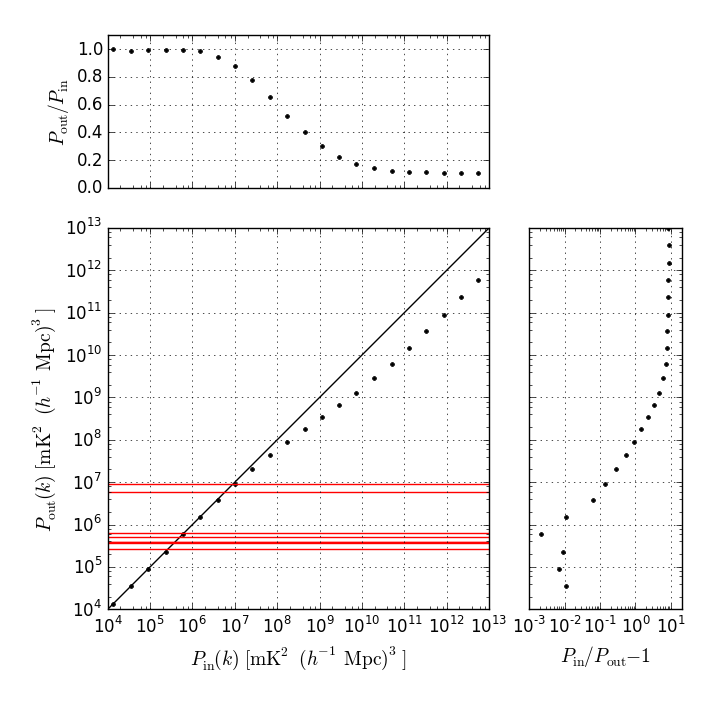
\includegraphics[width=\columnwidth]{plots/sigloss.png}
\caption{
Recovered power spectrum signal as a function of injected signal amplitude.  Shaded regions
indicate the range in measured amplitude of power spectrum modes in Figure \ref{fig:final_pspec}.  
Error bars indicate 95\% confidence intervals as determined from the Monte Carlo simulations
described in Section \ref{sec:sigloss}.
Because
the recovered signal amplitude is a monotonic function of the injected signal amplitude,
it is possible to invert the effects of signal loss in the measured power spectrum values
to infer the true signal amplitude on the sky. Over the range of powers measured, the 
maximum correction factor $P_{\rm in}/P_{\rm out}$ is less than 1.02 at 97.5\% confidence.
The transition to significantly higher correction factors at larger signal amplitudes
occurs as the injected signal
dominates over the foreground modes present in estimates of the data covariance.
}\label{fig:signal_loss}
\end{figure}


%\subsubsection{Integrating $k$-modes}
%XXX This shows the efficacy of using the median over the mean.
%The power spectrum shown in figure \ref{fig:final_pspec} is an average of
%multiple baselines together. To show how the modes in each power spectrum
%integrate together and to what degree they integrate down as noise are not, an
%allan variance test, is shown in Figure \ref{fig:pspec_variance}. Color
%represents a different $k$ mode measured in $\Delta^{2}$ along with the
%different bootstraps. Here we are showing the effect of integrating down on
%different $k$ modes as we include a wider range in time, and hence more
%independent modes. From the discussion on optimal fringe rate filtering we know
%we have 2 independent modes on the sky per LST hour. Hence, integrating modes
%upto a thousand modes, where not all are independent we expect to hit up against
%a floor, which we see. These curves are plotted for $P(k)$ and therefore, the
%colors represent both positive and negative $k$'s with green curves haveing the
%highest absolute value for $k$ and blue curves are modes closer to the horizon.
%
%
%We see a slight difference in the mean and median statistic when estimating the
%total value of modes. Modes tend to level off for both the statistcs and the
%amount of independent modes is capped when modes flatten out at roughly ~60
%samples. We find that this is close to the number of independent modes on the
%sky and baselines. In addtion modes close to the horizon (blue) tend to flatten
%out with the mean statictic, however there is an increased spread for the median
%statistic. 
%
%In addtion there is a sharp decline in power when integrating ~1024 modes for
%certain modes when dealing with the mean and median statistic. These modes show
%unexpected behaviour due to the sharp slope of the fall in power. Further
%investigation of these modes is to be conducted.
%


%
%   -PLOTS:
%       --example covariance matrices (with foregrounds, without, fringe rate
%         filtering.
%       --Before and After covariance application waterfall plots.
%
%       --Eigen Spectra and shape of the eigen modes.
%
%       --Window Functions : not waterfalls.
%
%       --Fisher matrices.
%
%       --Power spectrum waterfall plots for different separations. 
%
%       --Maybe the wedge.
%



%\section{Summary of Improvements from PSA32}
% Should this section be here? [ARP: no, it is now in discussion]
%In comparison to the previous PAPER pipeline (see \cite{parsons_et_al2014a}),
%this analysis took a slightly different approach which included some critical
%steps to improve our upper limit. In short, the improvements included using a
%new, refined redundant calibration method (Zheng 2014), increasing the width of
%the wideband delay filter that removes smooth spectrum foregrounds, weighting
%the lst binned data sets, and optimal fringe rate filtering. In section
%\ref{sec:calib}, we dicuss each of the improvements in more detail.
%
%Figure \ref{fig:step_through_pspec} (TBD) shows the power spectra when each of
%the steps mentioned above are turned off and for the one where all of them are
%turned on. We can see the gradual improvement of the power spectra (hopefully).


%%%%%%%%%%%%%%%%%%%%%%%%%%%%%%%%%%%%%%%%%%%%%%%%%%%%%%%%%%%%%%%%%%%%%%%%%%%%%%%%%%%


\section{Results}\label{sec:results}

\subsection{Power Spectrum Contstraints}

\begin{figure*}\centering
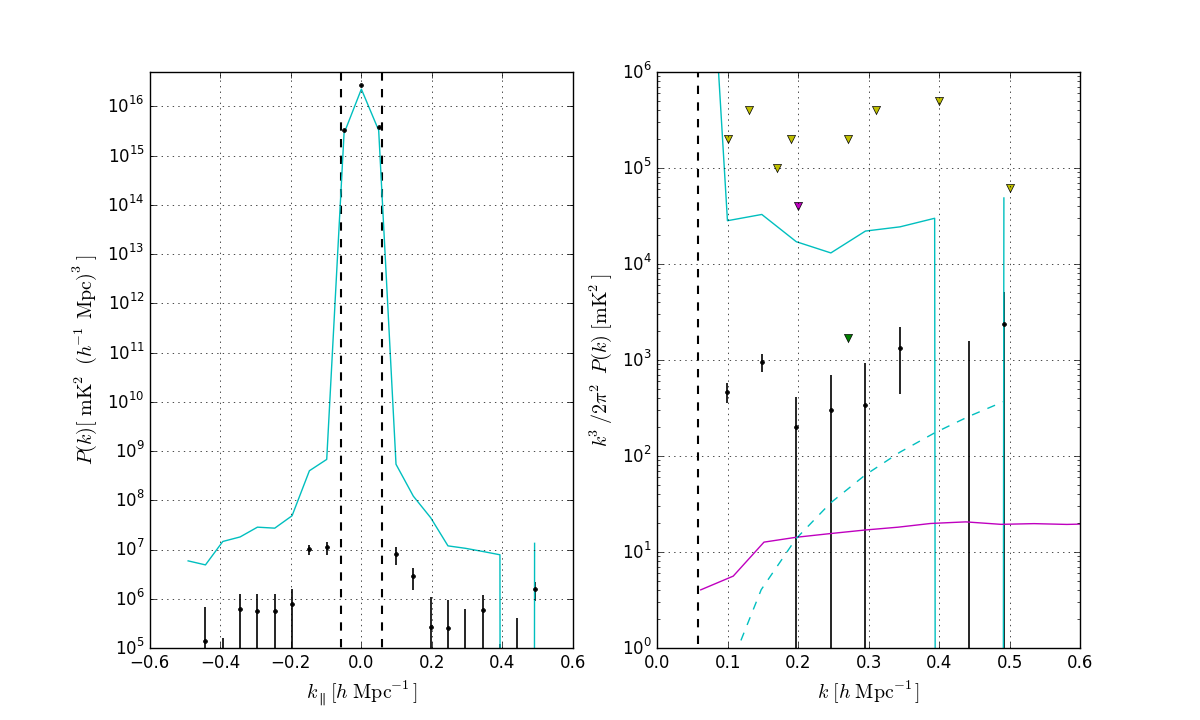
\includegraphics[width=2\columnwidth]{plots/pk_k3pk.png}
\caption{
Measured power spectrum (black dots with 2$\sigma$ error bars) at $z=8.4$
resulting from a 134-day observation with PAPER-64.  The dashed vertical lines
at $0.6\hMpci$ show the bounds of the delay filter described in Section
\ref{sec:wbd_filtering}. The theoretical $2\sigma$ thermal noise power spectrum
is shown in dashed cyan, assuming $\Tsys=500K$. The triangles indicate 2
$\sigma$ upper limits from GMRT \citep{paciga_et_al2011} (yellow) at $z=8.6$,
MWA \citep{dillon_et_al2013b} at $z=9.5$ (magenta), and the previous PAPER upper
limit (P14) at $z=7.7$. The magenta curve shows a predicted model 21 cm power
spectrum at 50\% ionization \citep{lidz_et_al2008}.
XXX Using 100 bootstraps. Correction factors are
fringe-rate filter (1.9), signal loss (1.02), and median statistic (1.4), delay
filter signal loss, bandpass signal loss.}
\label{fig:final_pspec}
\end{figure*}

Following the power spectrum analysis procedure outlined in Section \ref{sec:oqe_app},
we incoherently combine independent power spectrum measurements made at different
times and with different baseline groups using the median statistic.  As described
in Section \ref{sec:bootstrap}, we bootstrap over all of these independent measurements,
as well as over the selection of baselines included in the power spectrum analysis for
each baseline group, in order to estimate the error bars on the spherically averaged
power spectrum $P(k)$, where positive and negative $k_\parallel$ measurements
are kept separate for diagnostic purposes.  In the estimation of the 
dimensionless power spectrum
$\Delta^{2}\equiv{k^{3}P(k)}/{2\pi^{2}}$, the folding of $\pm k_\parallel$ is
handled along with the rest of the bootstrapping over independent modes.
Finally, the measured values for $P(k)$ and $\Delta^2(k)$ are corrected for signal
loss through all stages of analysis, as summarized in Table \ref{tbl:sigloss}.

The final results are plotted in Figure \ref{fig:final_pspec}.
For the first two modes outside of the horizon, we have
clear detections. We attribute these to foreground leakage from
inside the horizon related to the convolution kernels in equation \ref{eqn:delay_transform} (either
from the chromaticity of the antenna response, or from the inherent spectrum of the
foregrounds themselves).  Somewhat more difficult to interpret is the 
$3.0\sigma$ excess at $k\approx0.35\hMpci$, and to a lesser
degree, the $2.1\sigma$ deficit at $k\approx0.39\hMpci$.  The
latter may simply be a statistical fluctuation; we estimate a 19\% chance of 
a negative outlier at this significance occurring in the measurement of 11 modes, assuming
Gaussian statistics.  However, the outlier at $k\approx0.35\hMpci$ is
unlikely to be chance.

\begin{figure*}\centering
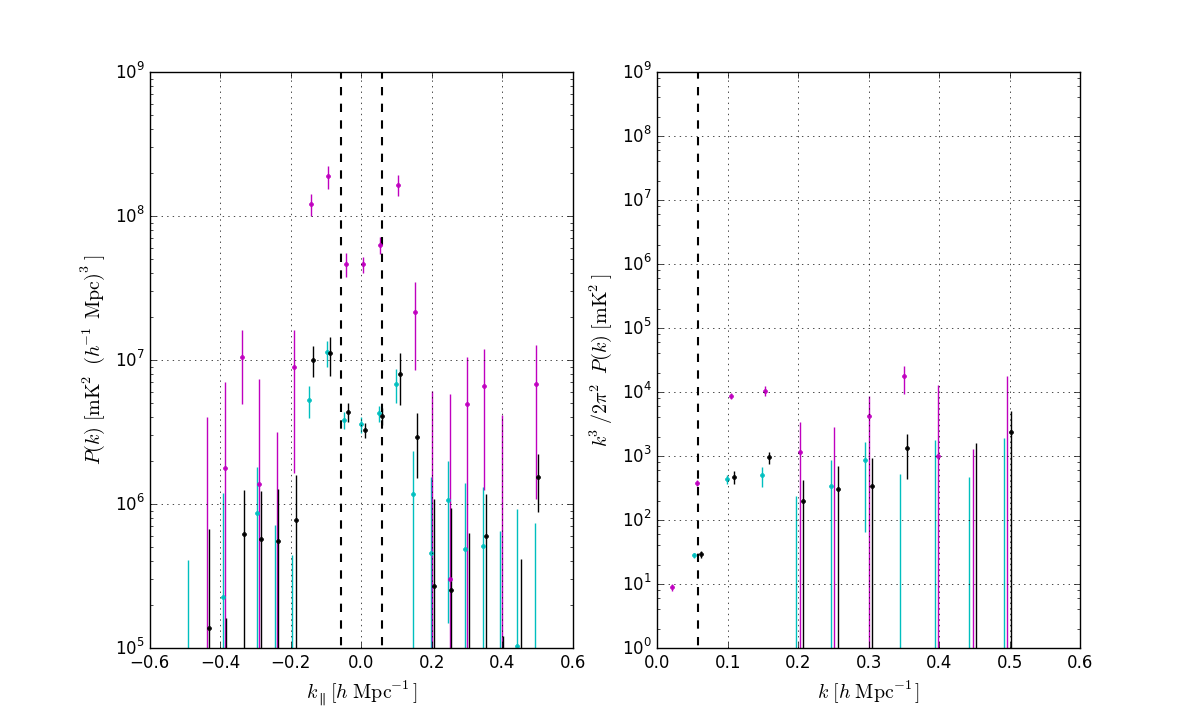
\includegraphics[width=2\columnwidth]{plots/pspec_comparison.png}
\caption{Diagnostic power spectra in the style of Figure \ref{fig:final_pspec}
illustrating the impact of various analysis stages.
Power spectra omitting the stages of fringe-rate filtering (magenta) and 
OMNICAL calibration (cyan) show higher residuals than the final power spectrum
(black) that includes both stages.
%The blue power spectrum has the full pipeline applied to it and is identical to
%\ref{fig:final_pspec}. The red power spectrum does not have omnical applied to
%it, and hence the error bars are bigger. Note that it does have the otimal
%fringe rate filter applied to it. Finally, the green power sepctrum does not
%have the optimal fringe rate filter applied.  However, it does have a fringe
%rate filter applied to that excludes negative fringe rates and those greater
%than the maimum fringe rate for the given baseline (east-west 30 m baselines). }
}\label{fig:pspec_comp}
\end{figure*}


We note that an excess centered at this wavemode was also
measured in P14 with an amplitude an order of magnitude higher.
In examining the effects on the power
spectrum of omitting various stages of analysis (see Figure \ref{fig:pspec_comp}), we
see that the excess is more pronounced in the magenta curve corresponding 
to the omission of fringe-rate filtering.
This suggests to us that the excess may be a result of foreground emission that is attenuated,
but not eliminated, in the current analysis.  
For example, the signal might be associated with
polarization leakage from a high rotation measure source near the horizon that
is attenuated by the spatial filtering achieved by the fringe-rate filter.
The absence of the excess in data without redundant calibration
(cyan) could be interpreted as indicating the excess is a modulation induced by frequency structure
in the calibration solution.  However, OMNICAL is constrained
to prohibit structure common to all baselines, so a more likely interpretation is that 
this faint feature decorrelates without the precision of redundant calibration.

\begin{figure}\centering
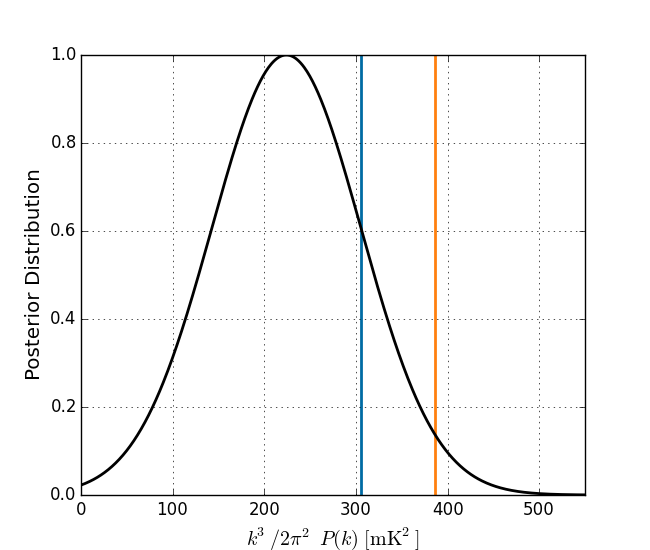
\includegraphics[width=\columnwidth]{plots/flat_k3pk_posterior.png}
\caption{Posterior distribution of power spectrum amplitude for a flat $\Delta^{2}$
power spectrum over $0.15<k<0.5\hMpci$ (solid black),
assuming Gaussian error bars. The blue and orange
vertical lines correspond to the 1$\sigma$ and 2$\sigma$ bounds, respectively.
The poseterior distribution excluding the the detection at $k=.35\rm \,hMpc^{-1}$ (dashed black) is shown for comparison.
}
\label{fig:final_posterior}
\end{figure}

In order to aggregate the information presented in the power spectrum into
a single upper limit, we fit a flat $\Delta^2(k)$ model to measurements
in the range $0.15<k<0.5\hMpci$.  We use a uniform prior of amplitudes between
-5000 and 5000 ${\rm mK}^2$, and assume measurement errors are Gaussian.
Figure \ref{fig:final_posterior} shows the posterior distribution of the fit.
From this distribution, we determine a mean of
$(15.0~{\rm mK})^2$ and a $2\sigma$ upper limit of $(19.7~{\rm mK})^2$. 
The measured mean is inconsistent with zero at the 2.7$\sigma$ level.
Even with the exclusion of the point at $k\approx0.35\hMpci$
(Figure \ref{fig:final_posterior}, dashed) the mean is inconsistent with
zero at $2.2\sigma$.

We conclude that we are likely beginning to 
detect a power spectrum excess at $k>0.15\hMpci$.  However, as illustrated
in Figure \ref{fig:pspec_comp}, the level of this excess appears to be
strongly dependent on fringe-rate filtering.  As discussed in \citet{parsons_et_al2015},
the normalization applied to $\Omega_{\rm eff}$ for fringe-rate filtering correctly
compensates for the effect of this filtering on power-spectral measurements
of an isotropic Gaussian sky signal.  We can surmise from the significant change in amplitude of the excess
under fringe-rate filtering that it arises from emission that violates these assumptions.
We conclude, therefore, that this excess is unlikely to be cosmic reionization, and is more
likely the result of non-Gaussian foregrounds.  As discussed earlier, one possible
culprit is polarization leakage \citep{moore_et_al2014,jelic_et_al2010,jelic_et_al2014}, although further
work will be necessary to confirm this.  It is worth noting that the interpretation of
the signal as polarization leakage is consistent with recent measurements in Stokes Q presented
in \citet{moore_et_al2015}.


To summarize, we believe the excess in our measured power spectrum is likely caused
by foregrounds.  Hence, we suggest ignoring the lower bound on the power spectrum amplitude
as not being of relevance for the cosmological signal.  Instead, we emphasize the 
2$\sigma$ upper limit of $(19.7~{\rm mK})^2$ at $z=8.4$, which significantly improves over the previous
best upper limit of $(41~{\rm mK})^2$ at $z=7.7$ reported in P14.  As we show below and in
greater detail in \citet{pober_et_al2015}, this limit begins to have significant ramifications
for the heating of the intergalactic medium prior to the completion of reionization.

\subsection{Spin Temperature Constraints}

\begin{figure*}\centering
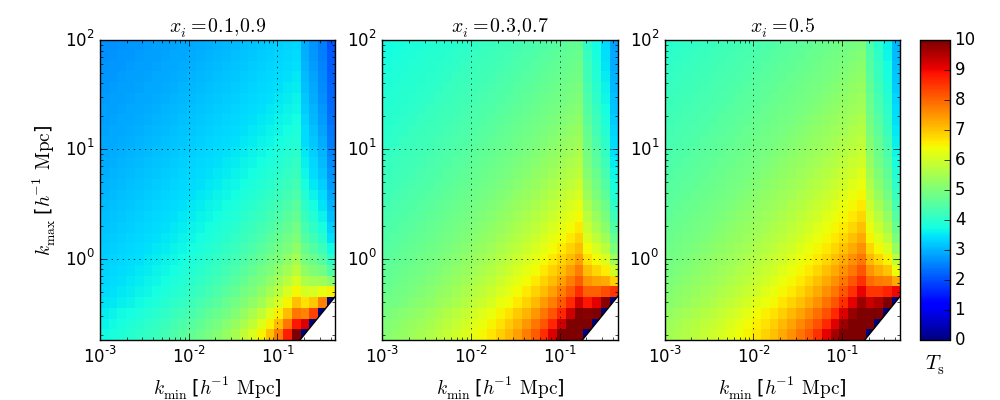
\includegraphics[width=2\columnwidth]{plots/ts_patchy_bound.png}
\caption{Constraints on the 21cm spin temperature at $z=8.4$, 
assuming 
the patchy reionization model in equations
\ref{eqn:d2pspec_model} and \ref{eqn:patchy_bound}, which hold in the limit
that $T_{\rm s}<T_{\rm CMB}$.
} \label{fig:patchy_bound}
\end{figure*}

In this section, we examine the implication of the measured upper limits
on 21cm emission in Figure \ref{fig:final_pspec} on the spin temperature
of the 21cm line at $z=8.4$.
In a companion paper \citet{pober_et_al2015}, we conduct a thorough analysis of the
constraints that can be put on the IGM using a simulation-based framework.
As a complement to that more thorough
analysis, we focus here on a simpler parameterization of the shape
of the 21cm power spectrum signal. 

The brightness temperature of the 21cm signal, $\delta{T_{b}}$, arising from the
contrast between the cosmic
microwave background, $\Tcmb$, and the spin temperature, $\Tspin$, is given
by 
\begin{equation}\label{eqn:tb}
    \delta{T_{b}} = \frac{\Tspin - \Tcmb}{1+z}(1-e^{-\tau})
\approx \frac{\Tspin - \Tcmb}{1+z}\tau,
\end{equation}
where temperatures are implicitly a function of redshift $z$, and
the approximation holds for low optical depth, $\tau$. 
The optical depth is given by \citep{zaldarriaga_et_al2004}
\begin{equation}\label{eqn:tau}
    \tau = \frac{3c^3\hbar A_{10} n_{\text{\tiny{HI}}}}{16k\nu_0^2\Tspin H(z)}
\end{equation}
%            %&\approx 8.6\times10^{-3}(1+\delta)x_{\text{\tiny{HI}}}\Big[\frac{T_{\gamma}(z)}{T_{s}}\Big] \Big(\frac{\Omega_{b}h^{2}}{0.02}\Big)\Big[\Big(\frac{0.15}{\Omega_{m}h^{2}}\Big)\Big(\frac{1+z}{10}\Big)\Big]^{1/2}
where $A_{10}$ is the Einstein A coefficient for the 21cm transition,
$n_{\text{HI}}$ is the density of the neutral hydrogen, $H(z)$ is the Hubble
constant, $x_{HI}$ is the neutral fraction of hydrogen, $\delta$ is the local
baryon overdensity, $\nu_0$ is the rest frequency of the 21cm transition, and 
the remainder are the usual constants.
%We ignore the effect of redshift space distortions.
Plugging in the cosmological parameters from \citet{planck_2015}, 
we get 
\begin{equation}\label{eqn:final_tb}
    \delta{T_{b}} \approx T_{0}\,x_{\text{\tiny{HI}}}\,(1+\delta)\, \xi ,
\end{equation}
where $\xi\equiv1-\Tcmb/\Tspin$ and $T_0\equiv26.7 \,
\text{mK} \sqrt{(1+z)/10}$.

If the spin temperature is larger than $\Tcmb$, we get the 21 cm signal in
emission with respect to the CMB, and $\xi\sim1$. However, if $\Tspin$ is less than $\Tcmb$,
$\delta T_b$ is negative and $\xi$ can potentially become large.
%The thermal history of the 21 cm line follows a very predictable theoretical
%model through cosmic time starting its journey by being coupled to the
%CMB temperature via compton scattering, There is no detectable 21 cm
%signal during this regime. 
%As the universe cools adiabatically, the gas temperature decreases as
%$T_K\propto(1+z)^2$ and colissional coupling puts the spin temperature below the CMB
%temperature and the 21 cm line reveals itself as an absorption feuture agains
%the CMB backdrop. Just before the first sources
%turn on to couple the spin temperature back to the
%gas temperature via the Wouthuysen-Field effect \citep{wouthuysen1952}, collsional coupling becomes
%inefficient and radiative coupling dominates, bringing the spin temperature in
%equilibrium with the CMB and there is no detectable 21 cm signal.
%Once the first sources turn on, the gas temperature
%becomes coupled to the spin temperature and the signal turns up in emission,
%after the heating of the gas by X-rays and blackhole accretion. 

As in P14,
we consider a ``weak heating" scenario in which $\Tspin$ is coupled to the gas temperature via
the Wouthuysen-Field effect \citep{wouthuysen1952,field1958,hirata2006},
but little heating has taken place prior to reionization, so that $\Tspin<\Tcmb$.
%\citep{wouthuysen1952}, but that there is no signicifcant source of heating
%from the usual suspects (X-ray binaries, blackhole accretion, etc...). 
%In this
%case, the 21 cm  signal will be in absorption, since $T_{s} < T_{\gamma}$.
In this scenario, 
because we have assumed little heating, we can approximate $\xi$ as having negligible spatial
dependence, and therefore $T_0^2\xi^2$ becomes a simple multiplicative scalar to the 
21cm power spectrum:
\begin{equation}\label{eqn:d2pspec_model}
    \Delta^2_{21}(k) = T_0^2\xi^2(z)\Delta_{i}^{2}(k),%\equiv
%\expval{T_{b}^{2}}\Delta_{i}^{2}(k),
\end{equation}
where $\Delta_{i}^{2}(k)$ is the dimensionless ionization power spectrum. 

As shown in P14, the maximum value of the
prefactor in equation \ref{eqn:d2pspec_model} is given by 
a no-heating scenario where the spin temperature follows the kinetic gas temperature,
which is held in equilibrium with the CMB via Compton scattering until $z_{\rm dec}\approx150$
\citep{furlanetto_et_al2006} and then cools adiabatically
as $(1+z)^2$.
In this case, $\xi$ is given by
\begin{equation}\label{eqn:maxxi}
\xi = 1 -\frac{1+z_{\rm dec}}{1+z} \approx -\frac{150}{1+z}.
\end{equation}
At $z=8.4$, this corresponds to a minimum bound on the spin temperature of $\Tspin>1.5~{\rm K}$.

We can now flip this argument around and, for a measured upper bound on $\Delta^2_{21}(k)$, we
can use models for $\Delta_i^2(k)$ in equation \ref{eqn:d2pspec_model} to place a bound
on $\Tspin$.  
%This produces a maximum prefactor of
%\begin{equation}
%    \text{max}[T_0\xi] \approx 370\left(\frac{10}{1+z}\right)^{1/2}~{\rm mK}.
%\end{equation}
%
%By rearranging equation \ref{eqn:d2pspec_model}, we get that 
%\begin{equation}
%    T_{b} = T_{0}(z)\xi(z) = T_{0}(z)(1 - \frac{T_{\gamma}}{T_{spin}},
%\end{equation}
%noting the fact that in our no heating scenario, the brightness temperature is
%negative. Solving for the spin temperature, we have that 
%\begin{equation}
%    T_{s}(z) = T_{\gamma}(z)\Big[1 - \frac{T_{b}}{T_{0}(z)}\Big]^{-1}.
%\end{equation}
We consider a class of ``patchy" reionization models (P12a,P14) which
approximates the ionization power spectrum as flat between minimum and maximum
bubble sizes, $\kmin$ and $\kmax$, respectively:
\begin{equation}\label{eqn:patchy_bound}
    \Delta^{2}_{i}(k) = (x_{\text{HI}} -
x_{\text{HI}}^{2})/\ln{(\kmax/\kmin)}.
\end{equation}
For combinations of $\kmin$ and $\kmax$,
we 
determine the minimum spin temperature 
implied by the $2\sigma$ 21 cm power
spectrum upper limits shown in Figure \ref{fig:final_pspec}.
Figure \ref{fig:patchy_bound} shows the results of these bounds
for neutral fractions of $x_{\text{HI}}=$ 0.1, 0.3, 0.5, 0.7, and 0.9.
In all cases, we find that $\Tspin\gtrsim 3\,\text{K}$, indicating 
that our measurements are inconsistent with the spin temperature
being coupled to a kinetic temperature governed strictly by
adiabatic expansion.

Our results become more interesting in the range of $\kmin\sim0.1$ and
$\kmax\sim30$ representative of fiducial simulations
\citep{lidz_et_al2008,zahn_et_al2007}.  For neutral fractions of 0.3, 0.5, and
0.7, we find that $\Tspin\gtrsim 5\,\text{K}$. \citet{pober_et_al2015} improves
on these results by using a simulation based framework, rather than relying on
the approximations used here. They show that the improved limits they find push
the bounds of the amount of heating possible given the currently observed star
formation rates in high-redshift galaxy populations
\citep{bouwens_et_al2014,mcleod_et_al2014} and assumptions about the
relationship between star formation rates and X-ray luminosities
\citep{furlanetto_et_al2006,pritchard_loeb2008,fialkov_et_al2014}.  Assuming the
midpoint of reionization lies close to $z=8.4$ (a reasonable assumption given
that \citealt{planck_2015} suggests a midpoint of $z=8.8$), both the bounds
found in this paper and \cite{pober_et_al2015}, show evidence for additional
sources of heating beyond the observed galaxy population.  We refer the reader
to \citet{pober_et_al2015} for a detailed examination of these results.


%%%%%%%%%%%%%%%%%%%%%%%%%%%%%%%%%%%%%%%%%%%%%%%%%%%%%%%%%%%%%%%%%%%%%%%%%%%%%%%%
%   -Tsys, and Tsys vs. time ?


%
%   -Final Pspecs and from various stages 
%       --before/after omnical: Data in
%           /data2/home/zakiali/psa_live/forlstbinning for the before data set.
%           Currently being binned.
%           Note that this data set has ~271 fewer files ~ 48 hours. Hence, it
%           is not the same as the omnical data set.
%           After data set is the one we have always been using : 
%           /data2/home/zakiali/psa_live/forlstbinning_omnical_2 :
%           lstbin_even and lstbin_odd.
%       --before/after frf. Ditto in the above directories.
%       --before after foregrounds. There is foreground data in there as well.
%       SHould we make a foreground run with the non omnical set as well.

%   -Future datasets. Things to look forward to.
%
%   -HERA
%
%   -Relative merrits of foreground avoidance vs fg filtering.
%
%   -relative importance of improvements of psa32.
%
%   -vamp on consistency with zero.
%
%   -Remaining challenges.
%
%       --Polarization leakage.
%       --Sensitivity 
%       --Seeing foregrounds.
%
%
%
%


%   -Implications for polarized foregrounds.
%       --Flip this around on David and James : We don't see anything at this
%         level, which implies such and such for polarized emission.
%   -Radio recombination and other unsmooth foregrounds. 
%       --paper by peng, Oh. We could maybe confirm this??
%   -Summarize Jonnie's Result.
%   -Repeat the science measurement in Parsons 2014. This will compliment the
%    Jonnies result.
%   -the wedge - maybe?



\section{Discussion}
%   -We now compare and contrast our result with those without some of the key
%   components of our analysis pipeline.
%
%   -First we consider the effect from omnical. 
%       -Applying a more precise calibration scheme increases the redundancy
%       between baselines. Hence, this decrease the noise in the measurement. 
%       -This is exactly what we see in the  final power spectrum measurement. 
%       figure \pspecfigure shows the power spectrum of data that has not had
%       omnical applied to it. THe error bars here are reduced by a factor of a
%       few. 
%
%   -Next we consider the effect of using an optimal fringe rate filter. 
%       -By applying an optimal fringe rate filter, we down weight fringe rate
%       bins that are less sensitive, and hence have less signal, and upweight
%       the more sensitive parts of the sky. 
%       -Figure \ref{fig:frf_pspec} shows the power spectrum with a naive fringe
%       rate filer, which is a flat filter and throws out the the fringe rates
%       outside of those possible for a baseline of the eor baselines used in
%       this analysis. 
%       -This gives us a sensitivity benefit of a factor of 3(XXX), as seen
%       in the figure. Note that this data does have omnical applied to it.
%

The improvement in our results over those in P14 are the result of four
major advances:
\begin{itemize}
\item the expansion of the PAPER array to 64 antennas doubled our instrument's power spectrum sensitivity,
\item using OMNICAL for redundant calibration significantly improved the clustering of measurements
over the previous implementation of LOGCAL used in P14,
\item fringe-rate filtering further improved power spectrum sensitivity by $\sim$50\% and suppressed
systematics associated with foregrounds low in the primary beam, and
\item moving from a lossless quadratic estimator targeting difference modes
in redundant measurements to an optimal quadratic estimator (with carefully calibrated signal
loss) significantly reduced contamination from non-Gaussian foregrounds.
\end{itemize}
Figure \ref{fig:pspec_comp} illustrates the effect of some of these advances on the final
power spectrum.
Other important advances include the use of the median statistic to reduce the impact
of non-Gaussian outliers in power-spectral measurements, and the use of a Cholesky
decomposition of the Fisher information matrix to help reduce leakage 
from highly contaminated modes within the wedge.

These new techniques and improvements to calibration have reduced the measured
bias in nearly all wavebands by an order of magnitude or more. 
The use of
OMNICAL to accurately calibrate the relative complex gains of the antennas has
shown to be a major improvement to the data-reduction pipeline. The accuracy and improvement of
this calibration brings redundant baselines into impressive agreement with one another
(see Figures \ref{fig:omniview} and \ref{fig:density}),
and provides important diagnostic information for
monitoring the health of the
array, flagging RFI events, and otherwise assessing data quality.
Fringe-rate filtering, which is described in greater depth in \citep{parsons_et_al2015}, is also
proving to be a flexible and powerful tool for controlling direction-dependent gains and
improving sensitivity.  If indeed the low-significance excess in the measured power spectrum
is coming as a result of polarization leakage, independent filtering of the XX and YY polarizations
prior to summation has the potential to better match these polarization beams and further suppress 
the leakage signal implied by \citet{moore_et_al2015}.

The end result is a major step forward, both for PAPER and for the field of 21cm cosmology.
While we have not yet made a detection of the 21cm cosmological signal, our limits are
now within the range of some of the brighter models.  As discussed in \citet{pober_et_al2015},
another order of magnitude improvement in sensitivity will make 21cm measurements highly constraining.



%Here, we discuss the effect to the power spectrum if various stages of the
%analysis were kept out. Specifically, we will discuss the effects of using
%OMNICAL and optimal fringe-rate filtering vs. not using them. This will give a
%sense of how different analyses effect the power spectrum.
%
%The merits of using OMNICAL were described above and it has the effect of
%bringing redundant baselines into better agreement with one another by
%calibrating out the differences between them. With this picture, we expect
%that for the power spectrum, error bars should become tighter. That is the
%noise in the measurement would be reduced. Comparing $P(k)$ for data that has
%been OMNICAL calibrated vs data that has not, but does have the redundant
%calibration that was used in P14 applied to it, we see that
%the error bars have decreased. This is shown in figure \ref{fig:pspec_comp}.
%Note that the error bars shrink for the higher $k$-modes, the error bars for the
%2 modes outside of the horizon do not have this systematic reduction because of
%the wideband delay filter. The wideband delay filter is applied after the
%calibration solutions have been applied to the visibilities and the 2 modes
%outside of the horizon are artifacts of the foregrounds leaking outside of the
%horizon. 
%
%Optimal fringe-rate filtering is a new technique that we have employed in our
%analysis and the effect it has on the power spectrum is crucial, considering it
%has a sensitivity benefit of a factor of 2. First of all, this fringe-rate
%filter improves the SNR by a factor of 2 for PAPER, increasing the total
%sensitivity of our measurement. Briefly, the filter does this by up weighting
%parts of the sky that are illuminated by the primary beam and down weighting
%parts of the sky that contain more noise. This has the effect of de noising the
%data. Figure \ref{fig:pspec_comp} shows the effect of minimal fringe-rate
%filtering. The filter applied here is the same as described in P14.
%It evenly weights fringe rates from 0 to $f_{max}$,
%where $f_{max}$ is the maximum fringe rate possible for a given baseline and
%frequency, discarding negative fringe rates. As can be seen in figure
%\ref{fig:pspec_comp}, the power spectrum in $\Delta^{2}$ comes down by a factor of
%2-3. The two modes outside of the horizon, which are dominated by foregrounds
%and are clear detections, also come down. The fact that these come down, implies
%that the foregrounds are down in the beam possibly near the horizon. Therefore,
%the signal there is attenuated by the use of this fringe-rate filter. 
%
%It is interesting that at $k\approx.25$, we get a detection of something that
%wasnt there before. Foregrounds? probably low level systematics we are hitting
%up against. Going to take some convincing...

%\subsection{Remaining Challanges}
%
%The closer we get to a detection of the 21 cm EoR fluctuations, the more we need
%to know what the systematics can be and at what level they can come in at. One
%of the biggest challenges remaining, as mentioned above, is the limited
%sensitivity of current EoR experiments. Even with the full sensitivity of the
%PAPER array at full build out, there will only be a $1.65\sigma$ EoR detection
%with the current method of foreground avoidance to detect the power spectrum.
%With the complete optimist approach of working withing the wedge, there will be
%a $8.86\sigma$ detection of the 21 cm power spectrum \citep{pober_et_al2014}.
%However, the configuration of PAPER makes it difficult to localize sources for
%removal and makes it hard to work within the wedge. These sensitivity benefits
%are being addressed by second generation EoR experiments, whose goal is to
%characterize the 21 cm power spectrum at high redshifts.
%
%In addition to sensitivity limitations, foregrounds are also a challenge that
%needs to be met. The delay spectrum approach requires that foregrounds need to
%be spectrally smooth so that they are localized to inside the horizon. As seen
%from equation \ref{eqn:delay_transform}, this approach also requires the need to
%know your beam and bandpass very well to mitigate the effect of spreading power
%outside the horizon. The PAPER beam is both spatially and spectrally smooth
%\cite{pober_et_al2012}, but even small variations have the effect of
%making spilling power outside of the horizon. In addition to the beam, the
%major source of error is in the bandpass. The 9th order polynomial fit to the
%bandpass is strictly not just the bandpass but contains ripples imprinted by
%sources other than Pictor A. Therefore characterizing the true bandpass of the
%instrument is hard and largely unknown for PAPER.
%
%Finally, one of the possibly biggest challenges we face is that of polarization
%leakage due to Faraday rotation of polarized sources from Stokes Q into Stokes
%I \citep{jelic_et_al2010,jelic_et_al2014}. 
%Through simulations, \cite{moore_et_al2013} showed that the expected
%polarization leakage at $z=8.5$ in $\Delta^{2}$ is between
%$10^{3}-3\times10^{3} (mk^{2})$ at $k\approx0.15\hMpci$. 
%[XXX careful with this comparison, since it is about to be revised downward in new moore et al paper]
%Our measured Stokes
%I power spectrum in figure \ref{fig:final_pspec} shows that we just on the cusp
%of seeing polarization leakage and possibly even ruling out some of the models
%used. [XXX i don't think this statement is backed up by the data]
%There might even be possible detection of the polarization leakage and
%would require us to move up in frequency to higher redshift where polarization
%is less prominent due to the $\lambda^{2}$ dependence of Faraday rotation.
%However, if we were seeing polarization leakage at $k\approx0.15\hMpci$, we
%would expect to see leakage at the higher $k_{\parallel}$ in our power spectrum
%since polarization leakage grows monotonically in $k$, for the modes we measure.
%We can conclude the this detection at $k=.15$ is just foreground leakage from
%within the horizon or some other systematics.
%
%For more sensitive arrays, like HERA and the SKA, polarization leakage may play
%a big problem and would require mitigation contingencies. One of the main ways
%that polarization leakage occurs is from elliptical beams, and hence a mismatch
%between the X and Y beams (for a crossed linear dipole design). Therefore, one
%way of mitigating the effects of polarization leakage is to design the
%instrument such that the beams are more circularly symmetric and therefore the
%mismatch between the X and Y polarizations is minimized. For PAPER this mismatch
%is expected to be at roughly $10\%$, which was used in the simulations in
%\cite{moore_et_al2013}.  The EoR signal is expected to be in the 10's of mK, and
%since these second generation instruments have the ability to make detect EoR
%with very significant confidence, the need to mitigate the polarization leakage
%effects, which may be up to 2 orders of magnitude brighter than the EoR signal,
%is a necessity.

%%%%%%%%%%%%%%%%%%%%%%%%%%%%%%%%%%%%%%%%%%%%%%%%%%%%%%%%%%%%%%%%%%%%%%%%%%%%%%%%%%



\section{Conclusions}\label{sec:conclusion}
We have shown a new upper limit on the 21 cm reionization power spectrum at $z=8.4$,
showing an almost an order of magnitude of improvement from the previous result (P14).
We found the $2\sigma$ upper limit of 425 $mK^{2}$ by fitting a
flat power spectrum in a $k$ range from $.15<$k$<0.5\hMpci$ to the
dimensionless power spectrum, $\Delta^{2}$. Using these limits we have improved
the limits on the 21 cm mean brightness temperature set in P14.

We also continue to demonstrate the efficacy of using delay filters for
foreground suppression and the foreground avoidance technique in measuring the power
spectrum. In addition, we employ novel techniques in this analysis and show that
the necessity of precise calibration is needed to make accurate and believable
measurements of the 21 cm reionization power spectrum. We also show that the use of beam
weighted measurements in the optimal fringe-rate filter is critical to
increasing sensitivity for instruments with natively low sensitivity due to
collecting area, increasing the SNR on the measurement by a factor of at least 2.
We have also demonstrated the stability of the PAPER instrument both in time and
between redundant baselines, showing that baselines agree on the same sky up to
systematical errors and that the time correlation between days is low in the
noise.

At the achieved levels of the power spectrum, we also put constraints on the
amount polarization leakage that could possibly corrupt the Stokes I power
spectrum. We show that polarization leakage is not shown for most $k$-modes at
the level of $\sim10^{3}\ \text{mK}^{2}$. 

Furthermore, the analysis in this paper is extended in \citep{pober_et_al2015}
by showing the science implications of this upper limit. Given our measured
upper limit, They show that
we can rule out regions of spin temperature, $T_{s}$,
and neutral fraction, $x$, that are not consistent with this result. In
addition, they compare this result with current X-ray luminosity functions and
show that there are not enough X-ray sources to cause heating of the IGM at
$z=8.4$ that are consistent with these results.

Looking forward, the need for larger arrays with increased collecting area is
becoming a necessity. Proposed experiments such as the Square-Kilometer Array
(SKA) and the Hydrogen Epoch of Reionization Array (HERA) are set to fill this
need. HERA is a collaborative experiment dedicated to detect and characterize
the 21 cm reionization power spectrum as well as eventually image the ionizing bubbles
from the formation of the first stars and galaxies. The HERA instrument
is proposed to be composed of a closely packed 547 element hexagonal array 
\citep{pober_et_al2014} with each element being a 14-m diameter
reflecting-dish, with a total array area of $\sim.1km^{2}$. Sensitivity forecasts
derived in \citet{pober_et_al2014} showed that HERA has the ability to
detect reionization at a significance between $\sim32\sigma$ to $\sim133\sigma$
depending on the foreground removal scheme used. The lower bound is for the
delay spectrum technique used in this paper, where modes within the horizon are
irrevocably corrupted, whereas the higher bound equates to when we can perfectly
work within the wedge. That is, it is possible to perfectly subtract sources
within the horizon.

PAPER itself is looking forward to 2 seasons of 128 antenna maximally redundant
configuration data set. This data set has to potential to increase  sensitivity
by a factor of $3.5$ as compared to the data set used in this paper. However,
due to constraints on the PAPER site in South Africa, the shortest baselines for
this array are $8\lambda$ (16m), instead of the $16\lambda$ (32m) baselines used
in this analysis, which may be riddled with systematics due to cross coupling
and reflections within the array. Therefore, only considering the 16 m
East-West baselines, there will be a total sensitivity benefit of $3$. However,
there is the potential to use the $48m$ nd $64m$ baselines in this analysis as
well, boosting the sensitivity to by another factor of 2. 

PAPER is continuing to integrate down toward the 21 cm signal and gaining ground
on overcoming challenges in systematics in the instrument as well being able to
look past foregrounds. Future work will again characterize the reionization power
spectrum over a range of redshifts and to measure directly the polarized power
spectrum. We also look forward to two seasons of 128 dual polarization PAPER
data which will increase the sensitivity of measurements by almost an order of
magnitude from the data used here. Also, construction of HERA is also under way,
which will have the sensitivity to make a $30\sigma$ detection of the 21 cm power
spectrum. We look forward to this.


%However, all major 21 cm experiments (LOFAR, MWA, and PAPER) are at the cusp of detection
%and all have the sensitivity to rule out the optimistic reionization scenarios.
% XXX don't put speculative stuff in intro
[XXX Might mention impact of wedge on predicted sensitivities.]
However, even with a detection from one of these experiments, a high signal-to-noise characterization of the 21 cm power spectrum and imaging of reionization will have to
wait until future 21 cm experiments such as the Hydrogen Epoch of Reionization
Array (HERA) and the Square Kilometer Array (SKA), which will have more raw
collecting area and greater sensitivity \citep{pober_et_al2014}.

\section{Acknowledgements} 

PAPER is supported by grants from the National Science Foundation (NSF; awards 0804508,
1129258, and 1125558).  ARP, JCP, and DCJ would like to acknowledge NSF support
(awards 1352519, 1302774, and 1401708, respectively).
JEA would like to acknowledge a generous grant from the Mount Cuba Astronomical Association for
computing resources.
We graciously thank SKA-SA for site infrastructure and observing support. In
addition we would like to thank our South African interns Monde Manzini and
Ruvano Casper from Durban University of Technology (DUT), who helped build out
the array from 32 antennas to the 64 antennas this analysis was based on. 
We would like to thank Josh Dillon for helpful discussions on optimal quadratic
estimators. 

%\clearpage
%\nocite{*}
\bibliographystyle{apj}
\bibliography{biblio}

\end{document}

